%% ****** Start of file aiptemplate.tex ****** %
%%
%%   This file is part of the files in the distribution of AIP substyles for REVTeX4.
%%   Version 4.1 of 9 October 2009.
%%
%
% This is a template for producing documents for use with 
% the REVTEX 4.1 document class and the AIP substyles.
% 
% Copy this file to another name and then work on that file.
% That way, you always have this original template file to use.

%\documentclass[aip,graphicx]{revtex4-1}
%\documentclass[aip,reprint]{revtex4-1}

%\usepackage{graphicx}

%\draft % marks overfull lines with a black rule on the right
%\documentclass[pre,aps,floatfix,authordate1-4,twocolumn]{revtex4-1}
%\documentclass[pre,aps,floatfix,authordate1-4]{revtex4-1}

\documentclass[aps,prl,superscriptaddress,twocolumn]{revtex4}



%\documentclass[aps,prl,preprint,groupedaddress]{revtex4}

\usepackage{rotating} 
\usepackage{times}
\usepackage{graphicx}
\usepackage{setspace}
\usepackage{amsmath}
\usepackage{epstopdf}
\usepackage[obeyFinal]{easy-todo}
\usepackage{csquotes}

\begin{document}

% Use the \preprint command to place your local institutional report number 
% on the title page in preprint mode.
% Multiple \preprint commands are allowed.
%\preprint{}

\title{NMRlipids IV: Headgroup \& glycerol backbone structures, and cation binding in bilayers with PS lipids} %Title of paper

% repeat the \author .. \affiliation  etc. as needed
% \email, \thanks, \homepage, \altaffiliation all apply to the current author.
% Explanatory text should go in the []'s, 
% actual e-mail address or url should go in the {}'s for \email and \homepage.
% Please use the appropriate macro for the type of information

% \affiliation command applies to all authors since the last \affiliation command. 
% The \affiliation command should follow the other information.

\author{O. H. Samuli Ollila}
\email[]{samuli.ollila@helsinki.fi}
%\homepage[]{Your web page}
\affiliation{Institute of Organic Chemistry and Biochemistry,
Academy of Sciences of the Czech Republic, 
Prague 6, Czech Republic}
\affiliation{Institute of Biotechnology, University of Helsinki}

\author{NMRlipids collaboration \todo{Authorship query to be sent soon.}}
\affiliation{nmrlipids.blogspot.fi} 


% Collaboration name, if desired (requires use of superscriptaddress option in \documentclass). 
% \noaffiliation is required (may also be used with the \author command).
%\collaboration{}
%\noaffiliation

\date{\today}

\begin{abstract}
  % insert abstract here
  Primarily measured but also simulated NMR order parameters will be collected also for other than phophatidylcholine
  (these are discussed in NMRlipids I) headgroup. The information will be used to understand structural differences between 
  different lipid molecules in bilayers.
\end{abstract}

%\pacs{}% insert suggested PACS numbers in braces on next line

\maketitle %\maketitle must follow title, authors, abstract and \pacs

% Body of paper goes here. Use proper sectioning commands. 
% References should be done using the \cite, \ref, and \label commands


%\label{}
\section{Introduction}
Phosphatidylserine (PS) is the most common negatively
charged lipid in eykaryotic membranes.
PS lipids compose 8.5\% of total lipid weight of erythrocytes,
but the abundance varies between different organelles up to
25-35\% in plasma membrane \cite{lemmon08,leventis10,li14}.
Despite of the relatively low abundance, PS lipids
are important signaling molecules. They interact with
signaling proteins \cite{leventis10}, regulate
surface charge and protein localization \cite{yeung08}, and
induce protein aggregation \cite{zhao04,gorbenko06}.
Some domains spesifically interact PS lipids,
while others are attracted by general electrostatics and the
binding can be regulated by calcium \cite{leventis10}.
Therefore, the structural details
of lipid headgroups and the details of cation binding
are crucial for the PS mediated signaling processes.

Previous experimental studies have concluded that
PS headgroups have more rigid conformation than
phophocholines (PC) due to hydrogen bonding or
electrostatic interactions \cite{browning80,buldt81}.
Multivalent cations and Li$^+$ are able to form strong
dehydrated molecular complexes with PS lipids,
while monovalent ions interact more weakly with PS
containing bilayers \cite{hauser77,kurland79,hauser83,hauser85,feigenson86,mattai89,roux90,roux91}.
Dilution of bilayers with PC lipids makes PS headgroups
less rigid and reduces propensity for the formation of
strong complexes with multivalent ions \cite{browning80,buldt81,roux90,roux91}.


The structure of PS lipid headgroups and their 
interactions with ions have been studied with
various experimental methods and theoretical techniques \cite{roux90,melcrova16,??}.
However, the consesus has not been reached 
due to the difficulties to interpret the experimental data \cite{??} and
the inaccuracies in simulation models at the
headgroup region \cite{botan15,catte16,ollila16}.
Some studies propose that the negatively charged lipids
attract cations only due to the increase of local concentration
in the vicinity of membranes and that the binding constant of cations is similar
to zwitterionic and negatively charged lipids \cite{seelig90,sinn06,??}.
On the other hand, some studies propose specific binding of calcium directly to PS lipid
headgroups \cite{vernier09,boettcher11,??},
The NMR data proposes that the PS headgroup is more rigid than PC,PE or PG
headgroups, but more detailed interperetation has not been done.

%Details of negatively charged lipids and their interactions
%with ions and proteins have been experimentally analyzed with
%various spectroscopic methods \cite{borle85,macdonald87,roux90,seelig90,pan14,melcrova16,??}
%NMR \cite{seelig90,??}, scattering \cite{pan14,??} and fluorescence spectroscopy
%which are often complemented with classical MD simulations \cite{pan14,melcrova16,??}.


Headgroup and glycerol backbone C-H bond order parameters
calculated from MD simulations have been
recently used to interpret the lipid structures in NMR experiments
and to validate lipid structure and ion binding in simulations of
PC lipid bilayers \cite{botan15,catte16,ollila16,ferreira16}.
In this work we apply this approach to PS lipid headgroup
in order to elucidate the structural details and ion binding
to negatively charged lipids. The results are expected to elucidate
also PS mediated signalling events because 
glycerol backbone and headgroup structure and behaviour are similar
in model membranes and in bacteria \cite{gally81,scherer87,seelig90}.


%In NMRlipids I and II project we were looking for a MD model
%which would correctly reproduce headgroup and glycerol
%backbone structures and cation binding for PC lipid bilayers \cite{botan15,catte16}.
%Here we extend the same goal for lipids with negatively charged PS headgroup.
%Chemical structure of PS headgroup together with other common biological
%lipids is shown in Fig. \ref{lipids}.
%\begin{figure}[]




%  \centering
%  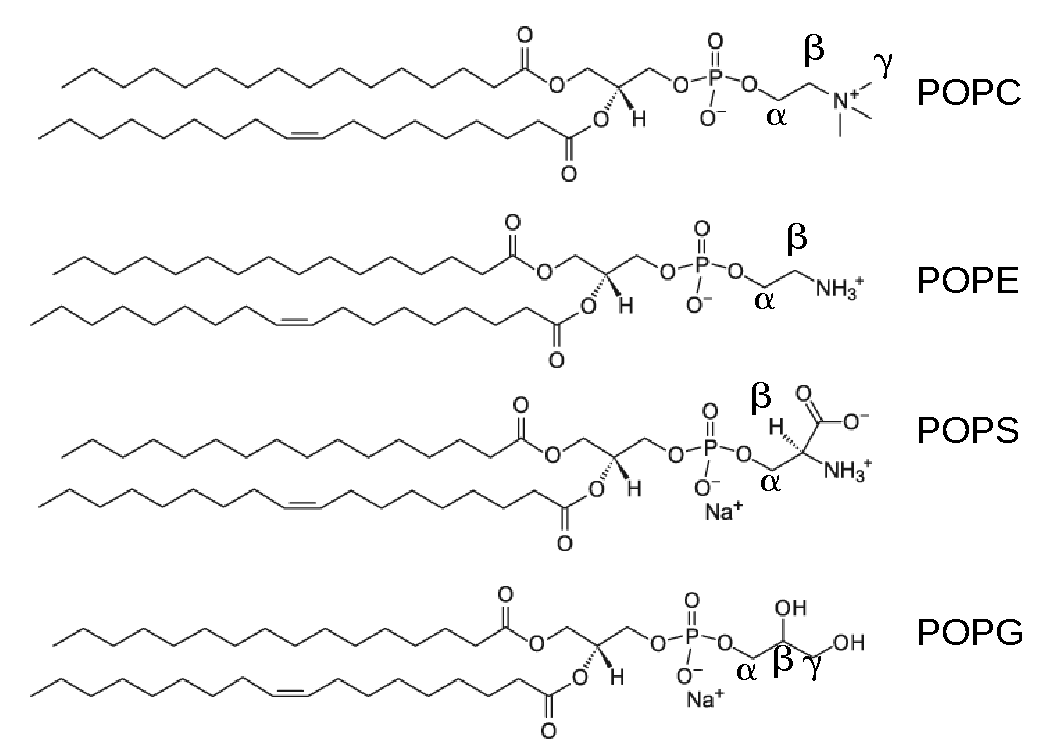
\includegraphics[width=9.0cm]{../Figs/lipids.pdf}
%  \caption{\label{lipids}
%    Chemical structures and labels for the headgroup carbons.
%  }
%\end{figure}


%The interpretation of this data and some other results has been that \cite{seelig90}
%\begin{displayquote}
%  {\it ''(i) Ca$^{2+}$ binds to neutral lipids (phosphatidylcholine, phosphatidylethanolamine) and negatively charged lipids
%    (phosphatidylglycerol) with approximately the same binding constant of K = 10-20 M$^{-1}$; \\
%    (ii) the free Ca$^{2+}$
%    concentration at the membrane interface is distinctly enhanced if the membrane carries a negative surface
%    charge, either due to protein or to lipid; \\
%    (iii) increased inter-facial Ca$^{2+}$ also means increased amounts
%    of bound Ca$^{2+}$ at neutral and charged lipids; \\
%    (iv) the actual binding step can be described by a Langmuir
%    adsorption isotherm with a 1 lipid:1 Ca$^{2+}$ stoichiometry, provided the interfacial concentration C$_M$, is
%    used to describe the chemical binding equilibrium.''}
%\end{displayquote}




%Phospholipids containing various polar headgroups and acyl
%chains are essential building blocks of biological membranes.
%Atomistic level structural details of lipids and lipid-ion 
%interactions are considered highly important in several
%biological processes. The lipid structure and ion binding
%can be studied in detail with NMR spectroscopy. However,
%the structural interpretation of NMR data requires usage
%of models. The combination of classical molecular dynamics
%simulations with NMR data, especially with C-H bond
%order parameters, can potentially give atomistic resolution
%interpretation of structure and dynamics of molecules \cite{botan15,ollila16,ferreira16}. 

%Our recent studies concluded that MD models are cabable to
%give structural interpretation for phosphatidylcholine 
%hydrophopic acyl chain region, while hydrophilic headgrop, glycerol 
%backbone and cation binding posed a major challenge for current
%force fields \cite{botan15,ollila16,catte16,ferreira16}. 
%These conclusions were reached by reviewing extensively 
%available experimental data from various sources and using
%NMRlipids Open Collaboration project to collect massive 
%amount of simulation data \cite{botan15,catte16}.

%Here we apply the same approach in search of MD simulation
%models which would reproduce glycerol backbone and 
%headgroup structures of lipids with PE, PG and PS headgroups.  
%In addition, we attempt to find a MD simulation model
%that would be able to correctly describe cation binding in
%bilayer containing negatively charged PG and PS lipids.


%Several MD simulation models have succesfully described 
%acyl chain structures and their qaulitative changes in different
%conditions for phosphatidylcholine lipids (for review see \cite{ollila16}).
%However, the current simulation models were not found to be accurate
%enough for full structural interpretation of phosphatidylcholine headgroup and
%glycerol backbone \cite{botan15}. Also Na$ +$  binding affinities
%were found to be significantly overestimated in several models and 
%none of the available models was able to Ca$2+$ 

\section{Methods}

\subsection{Solid state NMR experiments}
The magnitude and signs of the C-H bond order parameters in
headgroup and glycerol backbone were measured
using natural abundance $^{13}$C solid state NMR spectroscopy as
described previously \cite{ferreira13,ferreira16}.
Shortly, the absolute values of the order parameters were determined from the dipolar splittings
given by the indirect dimension of 2D R-PDFL experiment \cite{dvinskikh04} and
the signs were measured using S-DROSS experiments \cite{gross97}.

\todo{Details of the used spectrometer and maybe some other details should be given.} \\
\todo{Sample preparation should be described.} \\
\todo{How is the peak assignment done?}


\subsection{Molecular dynamics simulations}
Molecular dynamics simulation data was collected using
the Open Collaboration method \cite{botan15}.
The NMRlipids project blog (\url{nmrlipids.blogspot.fi}) and
the GitHub repository (\url{github.com/NMRLipids/NMRlipidsIVotherHGs})
were used as the communication platforms.
The simulated systems are listed in Table \ref{IONsystems} and
simulation details are given in the SI.
The simulation data is also indexed in the
searchable database (\url{nmrlipids.fi}),
and in the NMRlipids/MATCH GitHub repository (\url{https://github.com/NMRLipids/MATCH}).  
\begin{table*}[!htb]
%\begin{sidewaystable*}[!p]
\centering
\caption{List of MD simulations without additional salt.
   CKPM refers to the version with Berger/Chiu NH$_3$ charges compatible with Berger
   (i.e. the NH$_3$ group having the same charges as in the N(CH$_3$)$_3$ group of the PC lipids;
   'M' stands for Mukhopadhyay after the first published Berger-based PS simulation that used these charges)
   and CKP refers to the version with more Gromos compatible version
   (i.e. the charges for the NH$_3$ group taken from the lysine side-chain).
   %   these correspond the concentrations reported in the experiments by Akutsu et al.~\cite{akutsu81}.
   %   The lipid force fields named as in our previous work~\cite{botan15}.
}\label{IONsystems}
%begin{minipage}[t]{\textwidth}
\begin{tabular}{l c c r r r r r r c c}
  %\hline
  % some footnotes are not visible in typeset-MS (pdf)
 lipid/counter-ions & force field for lipids / ions & NaCl (mM) & CaCl$_2$\,(mM) &  \footnote{Number of lipid molecules with largest mole fraction}N$_{\rm l}$   &  \footnote{Number of water molecules}N$_{\rm w}$ \todoi{Should confirm that the amounts of water in experiments matched those in simulations.}   & \footnote{Number of additional cations}N$_{\rm c}$  & \footnote{Simulation temperature}T (K)  & \footnote{Total simulation time}t$_{{\rm sim}}$(ns) & \footnote{Time used for analysis}t$_{{\rm anal}}$ (ns) &   \footnote{Reference for simulation files}files\\
  \hline
    DOPS/Na$^+$  & CHARMM36 \cite{venable13}       &0 & 0 & 128 & 4480 & 0  & 303  & 500 & 100 & \cite{charmm36DOPS303K} \\
    DOPS/Na$^+$  & CHARMM36ua \cite{??} \todoi{Correct citation for CHARMMua DOPS}        &0 & 0        & 128 & 4480 & 0  & 303  & 500 & 100 & \cite{charmm36uaDOPS303K} \\
    DOPS/Na$^+$  & Slipids \cite{jambeck13}        &0 & 0        & 128 	& 4480  & 0  & 303  & 500 & 100 & \cite{slipidsDOPS303K} \\
    DOPS/Na$^+$  & Slipids \cite{jambeck13}        &0 & 0        & 288 	& 11232 & 0  & 303  & 200 & 100 & \cite{slipidsDOPSfiles} \\
    DOPS/Na$^+$  & Berger \cite{mukhopadhyay04}    &0 & 0        & 128  & 4480  & 0  & 303  & 500 & 100 & \cite{bergerDOPS303K} \\
    DOPS/Na$^+$  & GROMOS-CKP1 \cite{??} \todoi{Correct citation(s) for CKP.} &0 & 0  & 128 & 4480 & 0  & 303  & 500 & 100 & \cite{ckp1DOPS303K} \\
    DOPS/Na$^+$  & GROMOS-CKP2 \cite{??} \todoi{Correct citation(s) for CKP.} &0 & 0  & 128 & 4480 & 0  & 303  & 500 & 100 & \cite{ckp2DOPS303K} \\
    DOPS/Na$^+$  & lipid17 \cite{gould18} / JC  \cite{joung08} &0 & 0        & 128    & 4480   & 0   & 303  & 600 & 100 & \cite{lipid17DOPSjcions} \\
    DOPS/Na$^+$  & lipid17 \cite{gould18} / ff99 \cite{aqvist90}  &0 & 0        & 128    & 4480   & 0   & 303  & 600 & 100 & \cite{lipid17DOPSff99ions} \\
    \hline
    POPS/Na$^+$  & CHARMM36 \cite{venable13} &0 & 0 & 128 & 4480 & 0  & 298  & 500 & 100 & \cite{charmm36POPS298K} \\
    POPS/K$^+$   & CHARMM36 \cite{venable13} &0 & 0 & 128 & 4480 & 0  & 298  & 500 & 100 & \cite{charmm36POPS298Kpotassium} \\
    POPS/Na$^+$  & CHARMM36ua \cite{??} \todoi{Correct citation for CHARMMua DOPS}  &0 & 0 & 128 & 4480 & 0  & 298  & 500 & 100 & \cite{charmm36uaPOPS298K} \\
    POPS/Na$^+$  & Slipids \cite{jambeck13}        &0 & 0        & 128 & 4480 & 0  & 298  & 500 & 100 & \cite{slipidsPOPS298K} \\
    POPS/Na$^+$  & Berger \cite{??}        &0 & 0        & 128 & 4480 & 0  & 298  & 500 & 100 & \cite{bergerPOPS298K} \\
    POPS/Na$^+$  & MacRog \cite{maciejewski14}  &0 & 0        & ? & ?? & 0  & ?  & ? & ?  & \cite{??} \todoi{Data to be added by Piggot} \\
    OPPS/Na$^+$  & MacRog \cite{maciejewski14}  &0 & 0        & 128 & 5120 & 0  & 298  & 200 & 100 & \cite{macrogPOPS298K} \\
    POPS/Na$^+$  & GROMOS-CKPM \cite{??} \todoi{Correct citation(s) for CKP.} &0 & 0  & 128 & 4480 & 0  & 298  & 500 & 100 & \cite{ckp1POPS303K} \\
    POPS/Na$^+$  & GROMOS-CKP \cite{??} \todoi{Correct citation(s) for CKP.} &0 & 0  & 128 & 4480 & 0  & 298  & 500 & 100 & \cite{ckp2POPS303K} \\
    POPS/Na$^+$  & lipid17  \cite{gould18} / JC  \cite{joung08} &0 & 0        & 128    & 4480   & 0   & 298  & 600 & 100 & \cite{lipid17POPSjcions} \\
    POPS/Na$^+$  & lipid17 \cite{gould18} / ff99 \cite{aqvist90}  &0 & 0        & 128    & 4480   & 0   & 298  & 600 & 100 & \cite{lipid17POPSff99ions} \\
    \end{tabular}
%\end{minipage}
%\end{sidewaystable*} 
\end{table*}

\begin{table*}[!htb]
%\begin{sidewaystable*}[!p]
\centering
\caption{  List of MD simulations. The salt concentrations calculated as 
   [salt]=N$_{\rm c} \times$[water]\,/\,N$_{\rm w}$, where [water]\,=\,55.5~M.
   CKPM refers to the version with Berger/Chiu NH$_3$ charges compatible with Berger
   (i.e. the NH$_3$ group having the same charges as in the N(CH$_3$)$_3$ group of the PC lipids;
   'M' stands for Mukhopadhyay after the first published Berger-based PS simulation that used these charges \cite{??})
   and CKP refers to the version with more Gromos compatible version
   (i.e. the charges for the NH$_3$ group taken from the lysine side-chain).
   %   these correspond the concentrations reported in the experiments by Akutsu et al.~\cite{akutsu81}.
   %   The lipid force fields named as in our previous work~\cite{botan15}.
}\label{IONsystems}
%begin{minipage}[t]{\textwidth}
\begin{tabular}{l c c r r r r r r c c}
  lipid/counter-ions & force field for lipids / ions & NaCl (mM) & CaCl$_2$\,(mM) &  \footnote{Number of lipid molecules with largest mole fraction}N$_{\rm l}$   &  \footnote{Number of water molecules}N$_{\rm w}$ \todoi{Should confirm that the amounts of water in experiments matched those in simulations.}   & \footnote{Number of additional cations}N$_{\rm c}$  & \footnote{Simulation temperature}T (K)  & \footnote{Total simulation time}t$_{{\rm sim}}$(ns) & \footnote{Time used for analysis}t$_{{\rm anal}}$ (ns) &   \footnote{Reference for simulation files}files\\
  \hline
    POPC:POPS (5:1)/K$^+$  & CHARMM36 \cite{klauda10,venable13} &0 & 0  & 110:22 & 4935 & 0  & 298  & 100 & 100 \todoi{Equilibration?} & \cite{charmm36pops+83popcT298K}  \\
    POPC:POPS (5:1)/K$^+$  & CHARMM36 \cite{klauda10,venable13}          &0 & 0 & 250:50 & ?     & 0  & 298  & 200 & ?   & \cite{??} \todoi{Trajectories and further details to be added by J. Madsen}  \\
    POPC:POPS (5:1)/K$^+$  & CHARMM36 \cite{klauda10,venable13}          &0 & 0 & 110:22 & 4620  & 0  & 298  & 500 & 100 & \cite{charmm36pops+83popcT298Kpiggot}  \\
    POPC:POPS (5:1)/Na$^+$ & CHARMM36 \cite{klauda10,venable13}          &0 & 0 & 110:22 & 4620  & 0  & 298  & 500 & 100 & \cite{charmm36pops+83popcT298KpiggotSODIUM}  \\
    POPC:POPS (1:1)/K$^+$  & CHARMM36 \cite{klauda10,venable13}          &0 & 0 & 150:150 & ?    & 0  & 298  & 200 & ?   & \cite{??} \todoi{Trajectories and further details to be added by J. Madsen}  \\
     POPC:POPS (5:1)        & CHARMM36 \cite{klauda10,venable13,kim16}   &0 & 150 \todoi{Concentration to be checked} & 250:50 & ?  & ?  & 298  & 200 & ?  & \cite{??} \todoi{Trajectories and further details to be added by J. Madsen}  \\
    POPC:POPS (5:1)        & CHARMM36 \cite{klauda10,venable13,kim16}    &0 & 1000 \todoi{Concentration to be checked} & 250:50 & ?  & ?  & 298  & 200 & ?  & \cite{??} \todoi{Trajectories and further details to be added by J. Madsen}  \\
    \hline
    POPC:POPS\todoi{This is also probably OPPS? These should be corrected in this table as well.} (5:1)/K$^+$  & MacRog \cite{maciejewski14} &0 & 0  & 120:24 & 5760 & 0  & 298  & 200 & 200 \todoi{Equilibration?} & \cite{POPCpopsMACROG}  \\
   POPC:POPS (5:1)/K$^+$  & MacRog \cite{maciejewski14} &0 &100 & 120:24 & 5760 & 10  & 298  & 200 & 200 \todoi{Equilibration?} & \cite{POPCpopsMACROG}  \\
    POPC:POPS (5:1)/K$^+$  & MacRog \cite{maciejewski14} &0 &300 & 120:24 & 5760 & 31  & 298  & 200 & 200 \todoi{Equilibration?} & \cite{POPCpopsMACROG}  \\
    POPC:POPS (5:1)/K$^+$  & MacRog \cite{maciejewski14} &0 &1000 & 120:24 & 5760 & 104  & 298  & 200 & 200 \todoi{Equilibration?} & \cite{POPCpopsMACROG}  \\
    POPC:POPS (5:1)/K$^+$  & MacRog \cite{maciejewski14} &0 &3000 & 120:24 & 5760 & 311  & 298  & 200 & 200 \todoi{Equilibration?} & \cite{POPCpopsMACROG}  \\
    \todo{MacRog simulations with KCl to be added}\\
    \hline
    \todo{Berger simulations with NaCl and CaCl to be added}
\end{tabular}
%\end{minipage}
%\end{sidewaystable*} 

\end{table*}

The C-H bond order parameters were calculated directly
from the definition
\begin{equation}
S_{\rm CH}=\frac{1}{2}\langle 3\cos^2\theta -1 \rangle,
\end{equation}
where $\theta$ is the angle between the C-H bond and the membrane normal.
Angular brackets point to the average over all sampled configurations.
\todo{Error estimation should be discussed.}\\
The number density profiles were calculated using {\it gmx density} tool
from Gromacs sofware package \cite{gromacsMANUAL}.

\section{Results and Discussion}

\subsection{Headgroup and glycerol backbone order parameters measured from POPS lipid bilayer}

The INEPT and 2D R-PDLF experiments from POPS sample give well resolved spectras for all the
carbons in headgroup and glycerol backbone region, except for g$_3$ for which the resolution
was not sufficient to determine the numerical value of the order paramater (Fig. \ref{PShgSIGNSsimpson}).
Slices of the R-PDFL spectra (Fig. \ref{PShgSIGNSsimpson} C)) 
show a single splitting for the $\beta$-carbon with the order parameter value of 0.12,
and a superposition of a large and a very small splitting for the $\alpha$-carbon.
The larger splitting gives a order parameter value of 0.09, while the numerical value
from the small splitting cannot resolved with the available resolution.
Since only the absolute values of the PS headgroup order parameters were measured
previously \cite{browning80,roux91}, we used the S-DROSS experiment \cite{??} to determine the signs of
the order parameters. The S-DROSS slice for the $\beta$-carbon (Fig. \ref{PShgSIGNSsimpson} D)) clearly shows that the
order parameter is negative, which is confirmed by SIMPSON simulations.
The beginning of the S-DROSS slice suggests that the higher order parameter of
the $\alpha$-carbon is positive and the deviation towards negative values with the longer T$_1$ times suggests
that the smaller order parameter is negative. This is confirmed by a SIMPSON simulation
where the value of -0.02 was taken from $^2$H NMR experiment \cite{roux91} for the smaller order parameter.
The literature value was used because the
resolution of our experiment was not sufficient to determine the
small value of the order parameter. The S-DROSS curve from
SIMPSON simulation with a positive value for the smaller order parameter
(dashed grey in Fig. \ref{PShgSIGNSsimpson} D)) did not agree with the experiment, 
confirming the interpretation that the smaller order parameter is negative.
\begin{figure}[!htb]
  \centering
  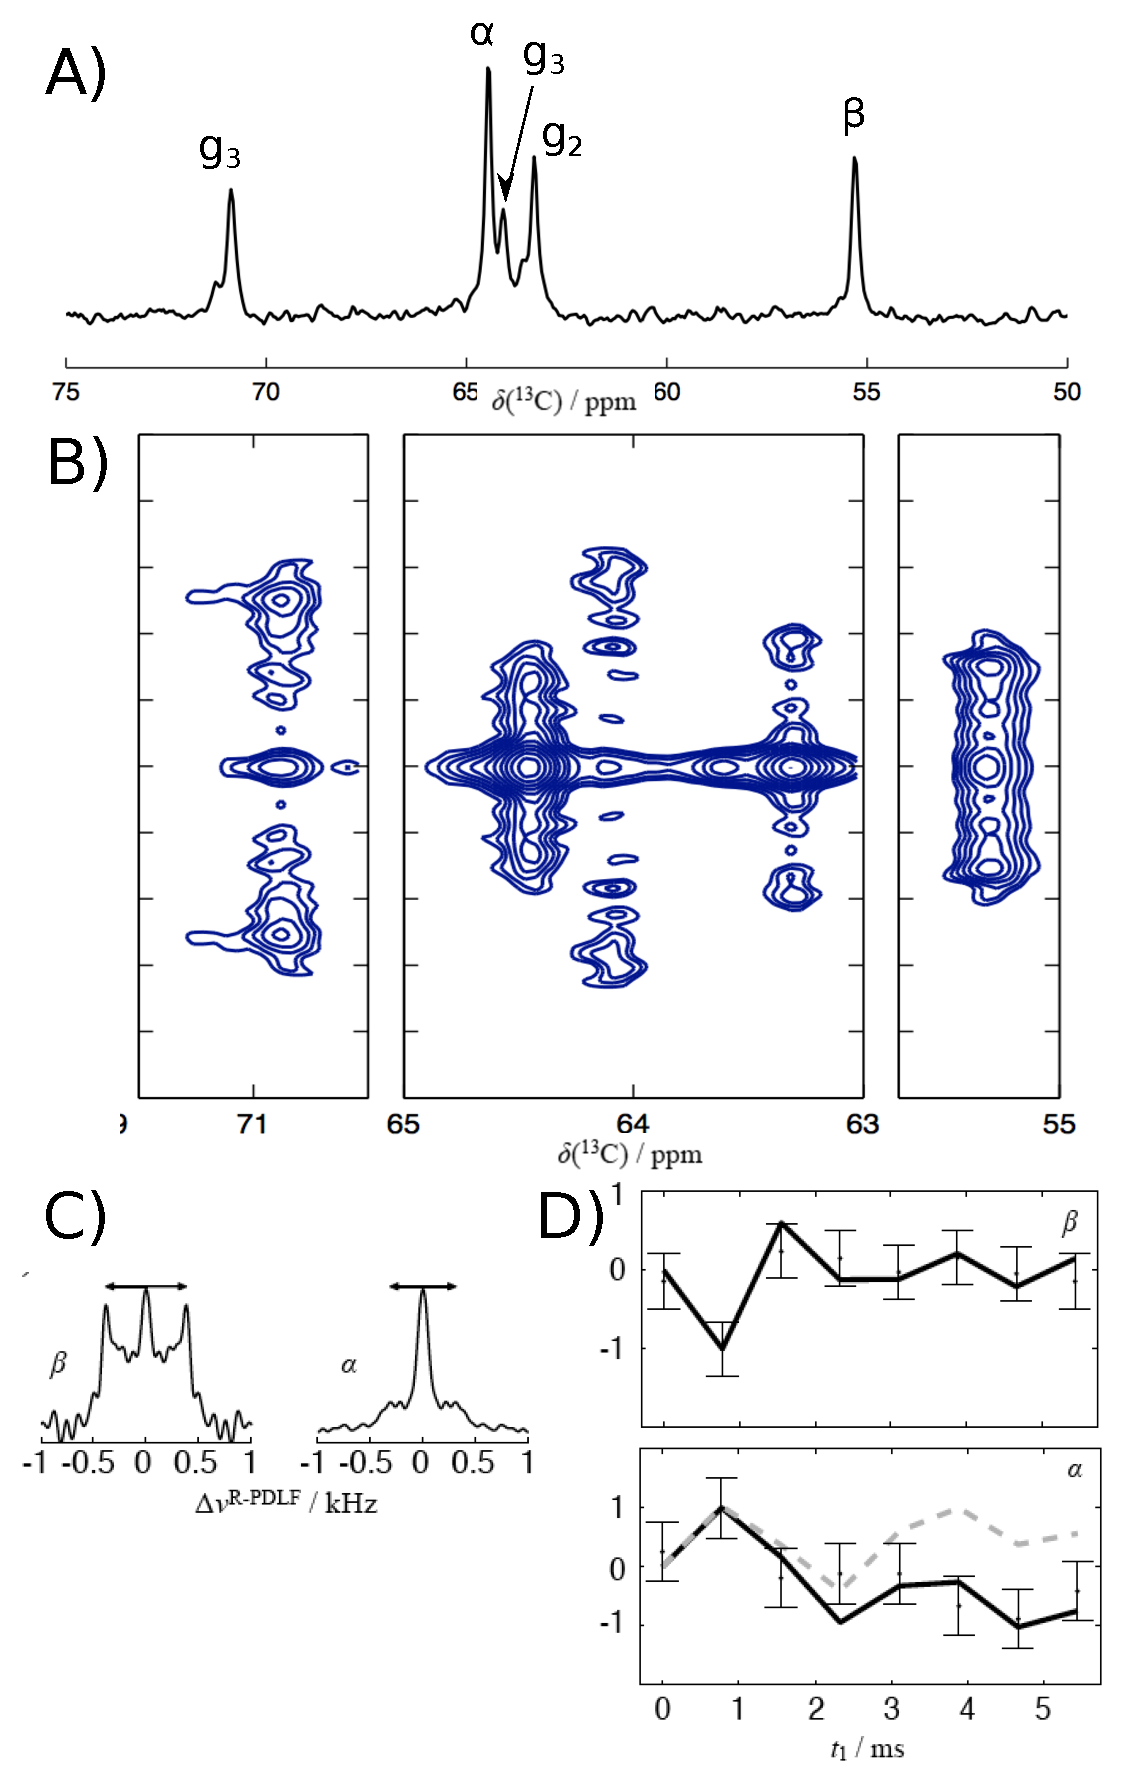
\includegraphics[width=8.5cm]{../scratch/figIDEA.eps}
  \caption{\label{PShgSIGNSsimpson}
    (a) The headgroup region of the INEPT spectrum with headgroup and glycerol backbone carbons assigned.
    (b) 2D R-PDLF spectra for headgroup and glycerol backbone regions.
    (c) Slices for $\alpha$ and $\beta$ barbons.
    (d) Experimental SDROSS data (points) and SIMPSON simulations (lines).
    Order parameter values of -0.12 for the $\beta$-carbon, and 0.09 and -0.02
    for the larger and smaller $\alpha$-carbon slittings were used in the
    SIMPSON calculations. The S-DROSS curve from SIMPSON simulation with positive value
    for the smaller order parameter (dashed grey).
  }
  \todo{This is preliminary figure, should be polished.}
  \todo{Should we show slices for all the analyzed carbons in (c)?}
\end{figure}

%\begin{figure}[!htb]
%  \centering
%  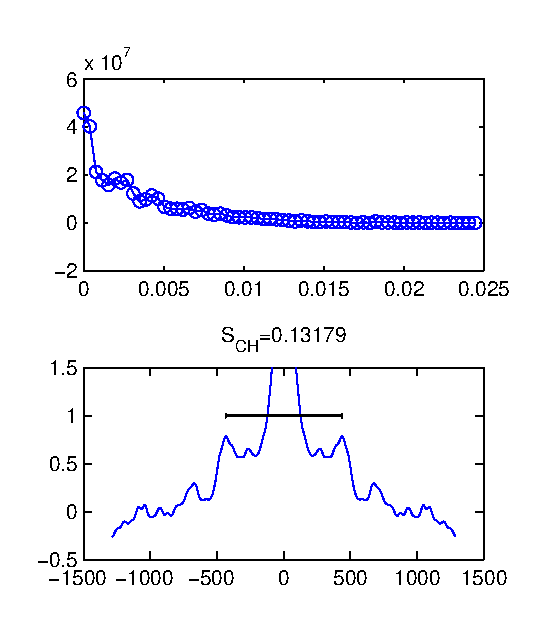
\includegraphics[width=5.5cm]{../Figs/g1_slice_large.eps}
%  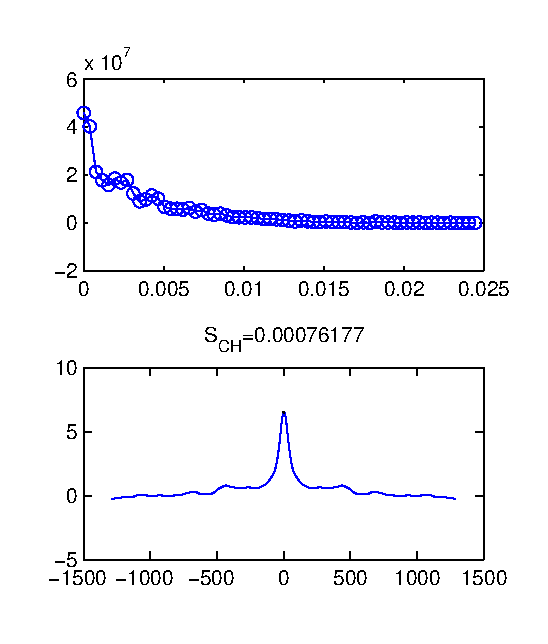
\includegraphics[width=5.5cm]{../Figs/g1_slice_small.eps}
%  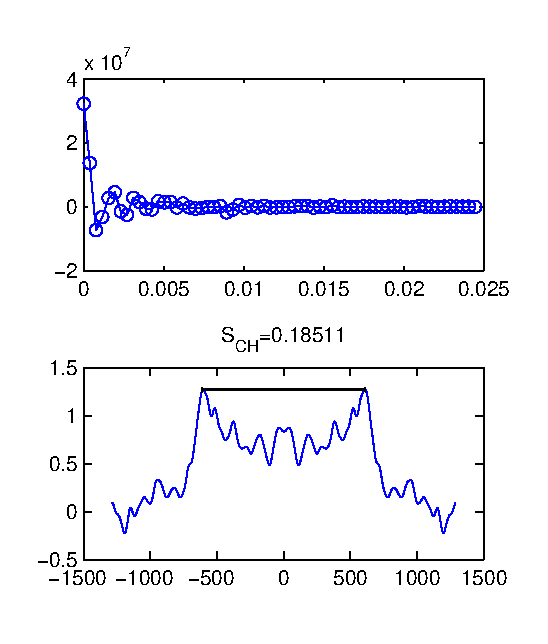
\includegraphics[width=5.5cm]{../Figs/g2_slice.eps}
%  \caption{\label{glycerolNMR}
%    R-PDFL slices for gycerol backbone carbons.
%  }
%  \todo{We need nicer figure for this data. Maybe combine with \ref{PShgSIGNSsimpson}} \\
%  \todo{What are the top figures actually?}
%\end{figure}

The headgroup and glycerol backbone order parameters of 
POPS measured in this work are in good agreement with the previously reported
values from $^2$H NMR experiments of DOPS \cite{browning80} (Fig. \ref{HGorderParameters}).
The $\beta$-carbon order parameter is significantly more negative and $\alpha$-carbon
experiences a significant forking in PS headgroup when compared with
the values previously measured for POPC \cite{ferreira13} (Fig. \ref{HGorderParameters}).  
These features have been intepreted to arise from a rigid PS headgroup
conformation, stabilized by hydrogen bonds or electrostatic
interactions \cite{browning80,buldt81}, but detailed structrural interpretation is not
available. 
%The detailed structural differences between the headgroups is, however, not known.
\begin{figure}[]
  \centering
  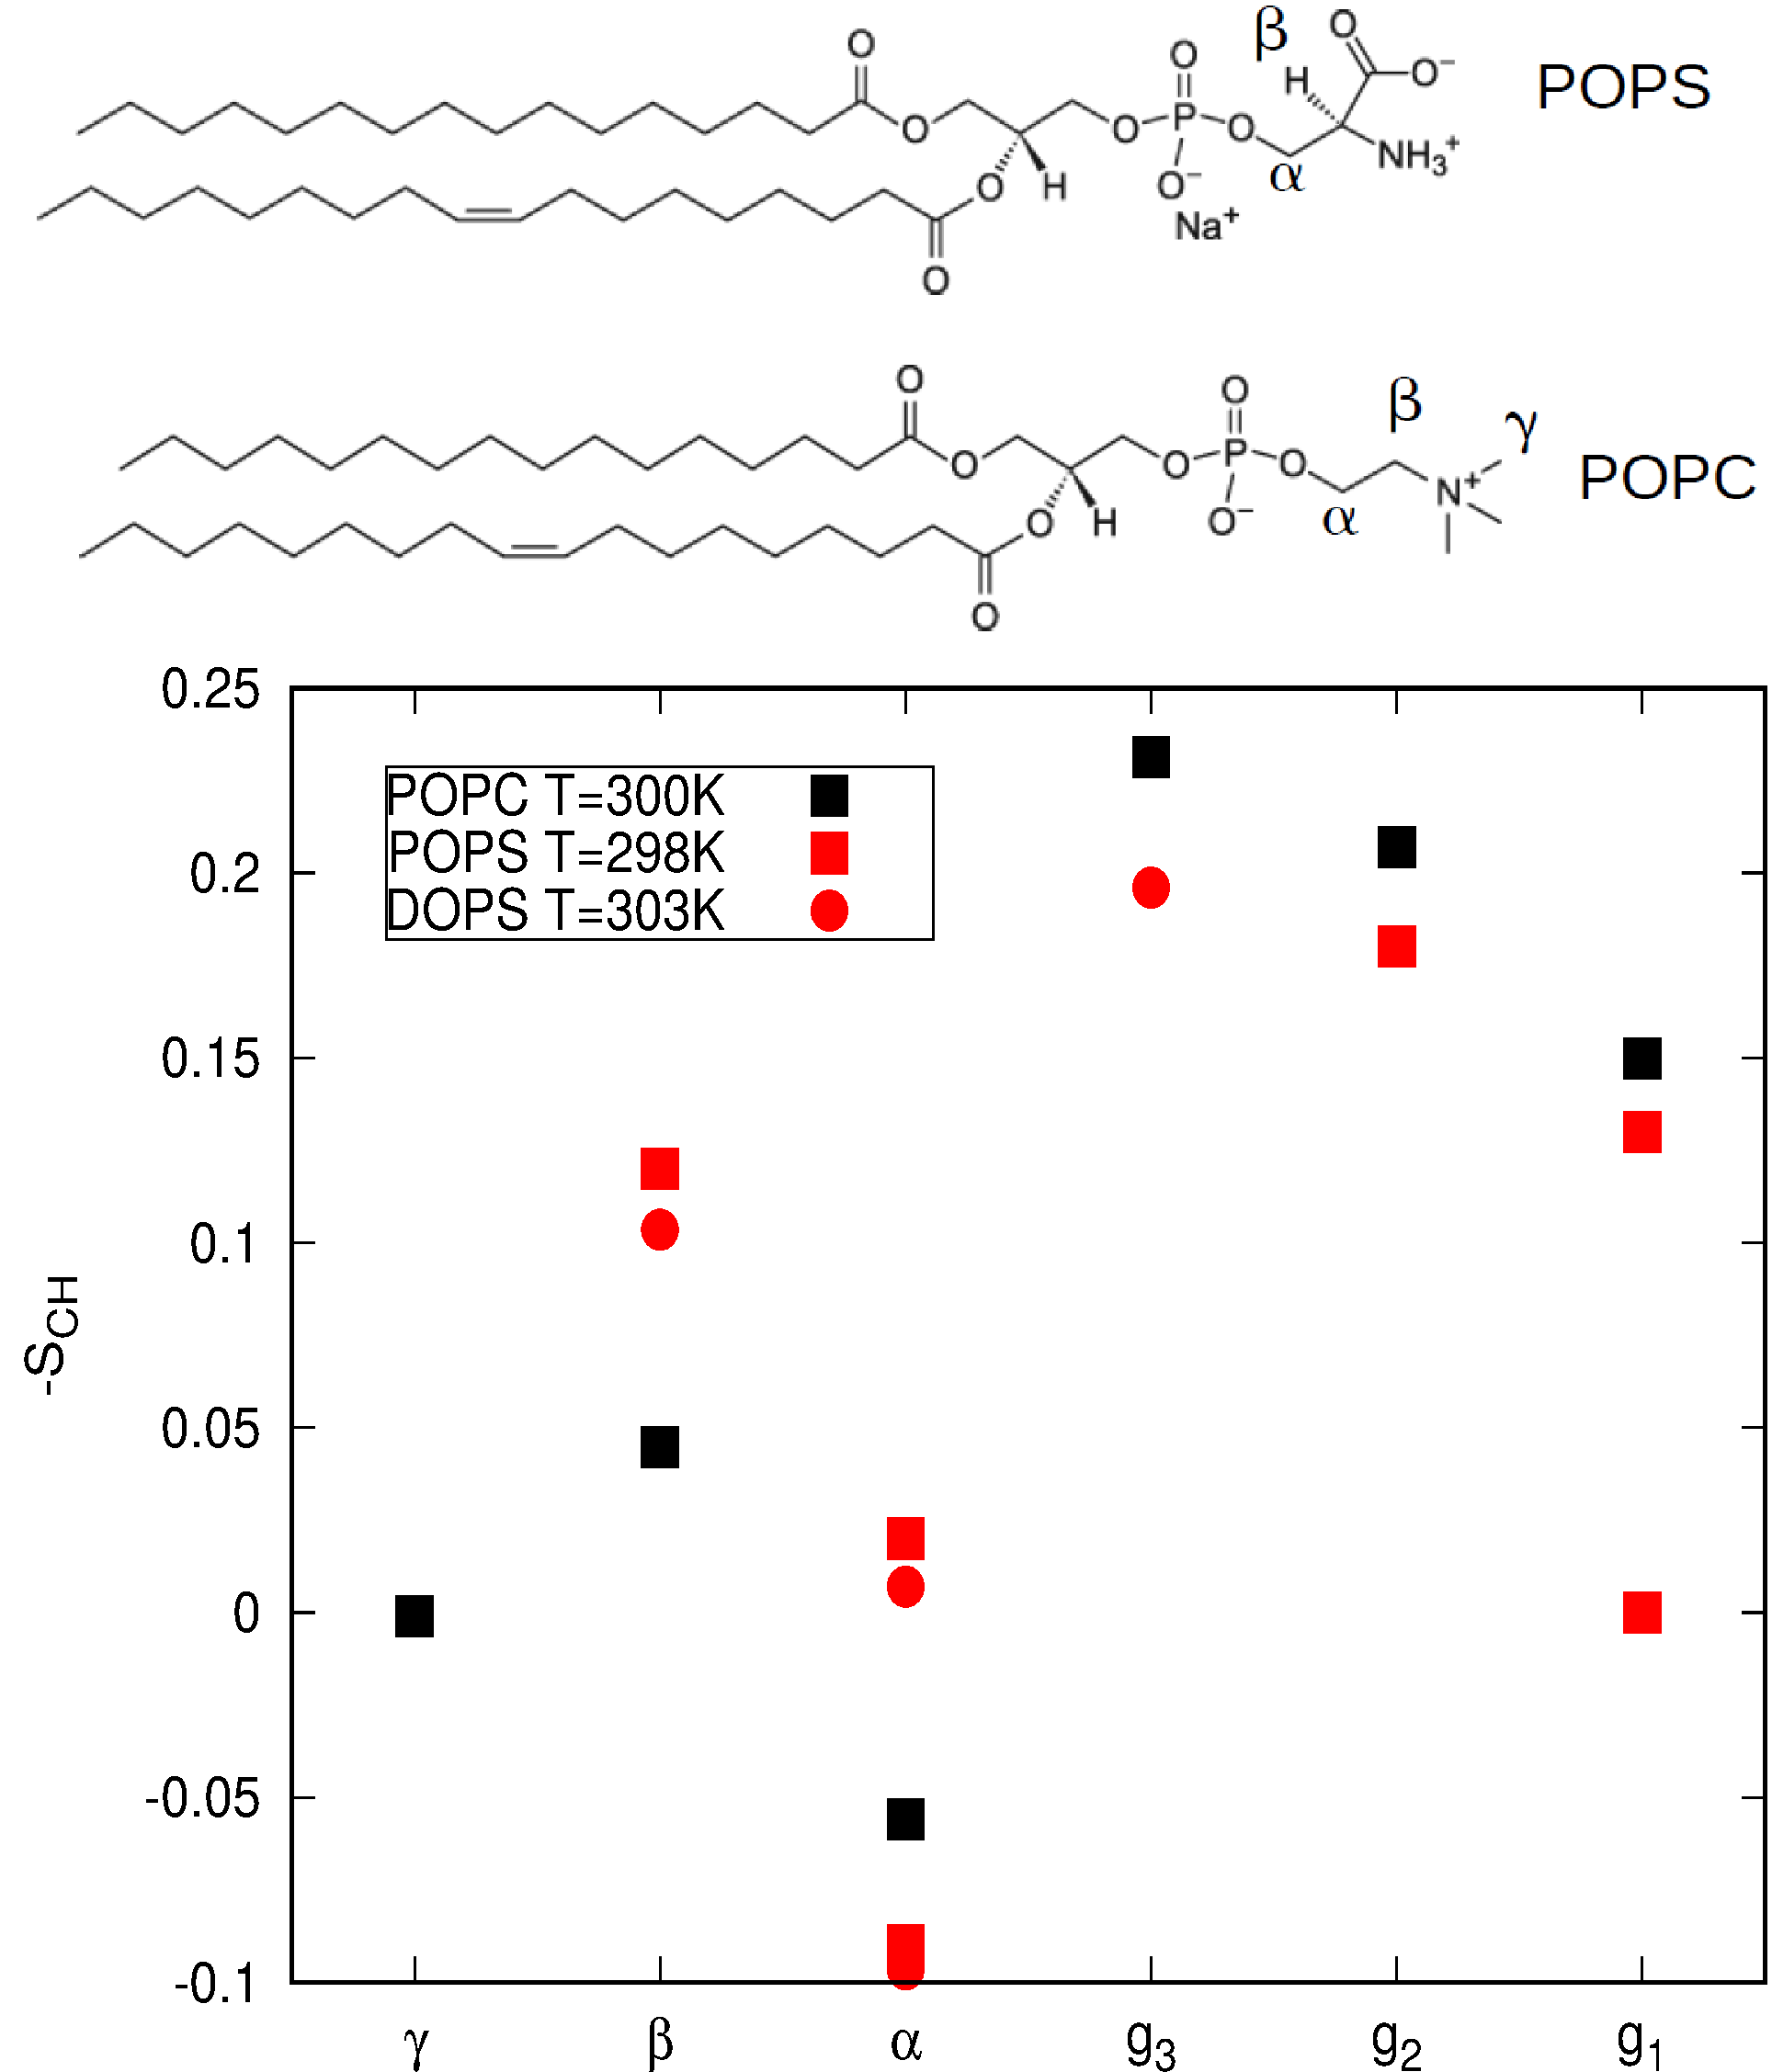
\includegraphics[width=9.0cm]{../Figs/PCPScomp.pdf}
  \caption{\label{HGorderParameters}
    Headgroup and glycerol backbone order parameters of POPS measured in this work compared
    with values for DOPS ($^2$H NMR, 0.1M of NaCl) \cite{browning80} and 
    POPC  ($^{13}$C NMR) \cite{ferreira13} from literature. Signs for PS order parameters
    as measured in this work and signs for PC as measured in Refs \cite{??,ferreira16}.
    %POPG from \cite{borle85} contains 10nM PIPES, DPPG from \cite{wohlgemuth80} contains  10mM PIPES and 100mM NaCl,
    %DPPE from \cite{seelig76}, E.coliPE and E.coliPG are from \cite{gally81}.
  }
  \todo{There should be values in \cite{roux90} which should be added.}
\end{figure}


%\begin{figure}[]
%  \centering
%  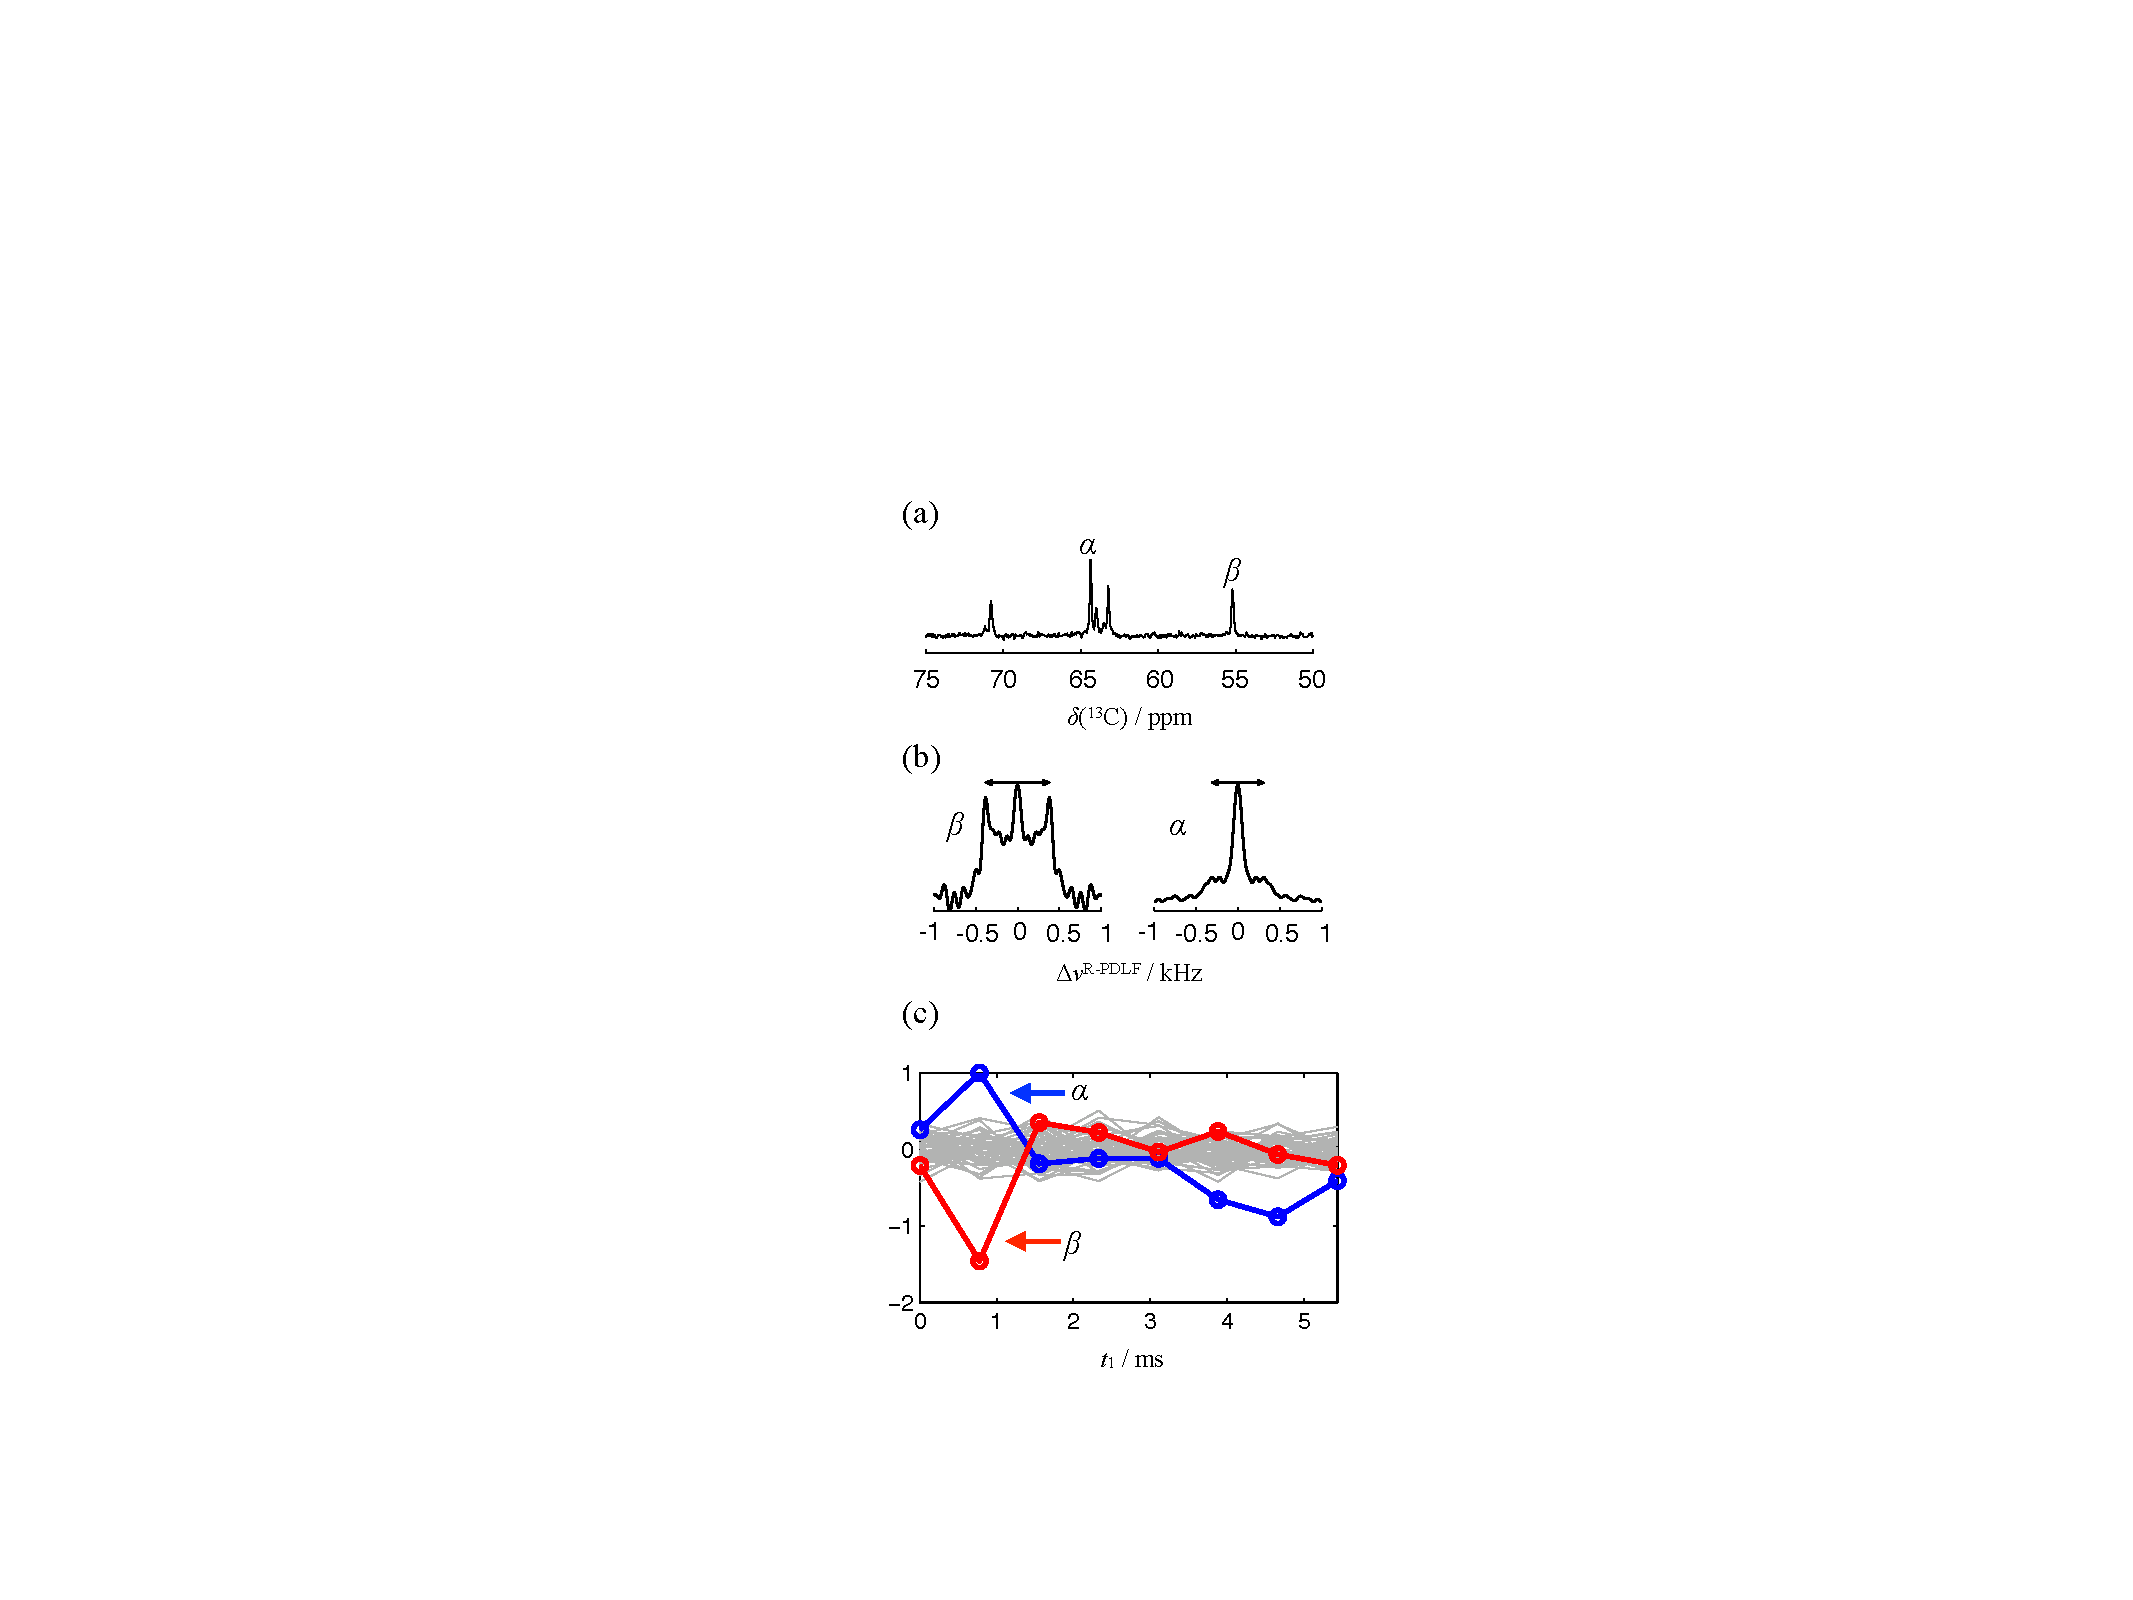
\includegraphics[width=9.0cm]{../Figs/PShgSIGNS.pdf}
%  \caption{\label{PShgSIGNS}
%    Experimental results for sign measurement for POPS sample
%  }
%\end{figure}


\subsection{Headgroup and glycerol backbone in simulations of PS lipid bilayers without additional ions}
\begin{figure}[]
  \centering
  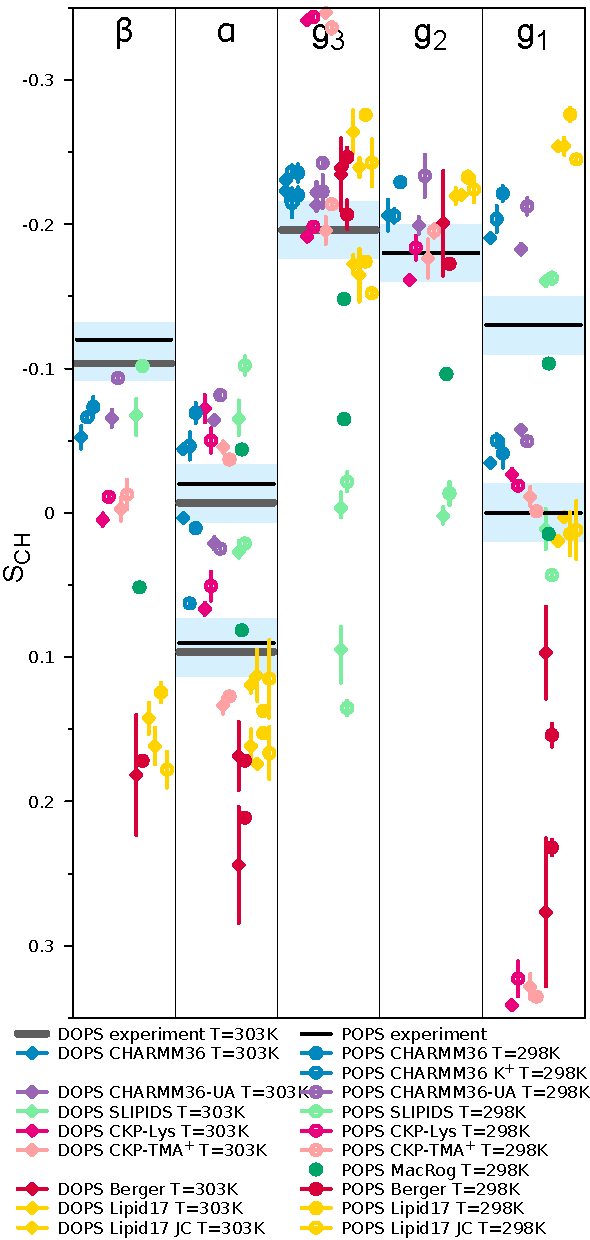
\includegraphics[width=9.0cm]{../Figs/HGorderparametersPS.pdf}
  \caption{\label{HGorderParametersPS}
    Order parameters for PS headgroup and glycerol
    backbone from simulations with different models and experiments without CaCl$_2$.
    All DOPS data at 303~K, POPS at 298~K.
    Experimental data from \cite{browning80} contain 0.1~M of NaCl.
    Signs are taken from experiments for POPS described in Supplementary Information.
    The vertical bars shown %for most computational values
    are not error bars, but demonstrate that %for these systems
    we had at least two data sets; the ends of the bars mark the extreme values from the sets, and the dot marks their measurement-time-weighted average.
  }
\end{figure}

\begin{figure}[]
  \centering
  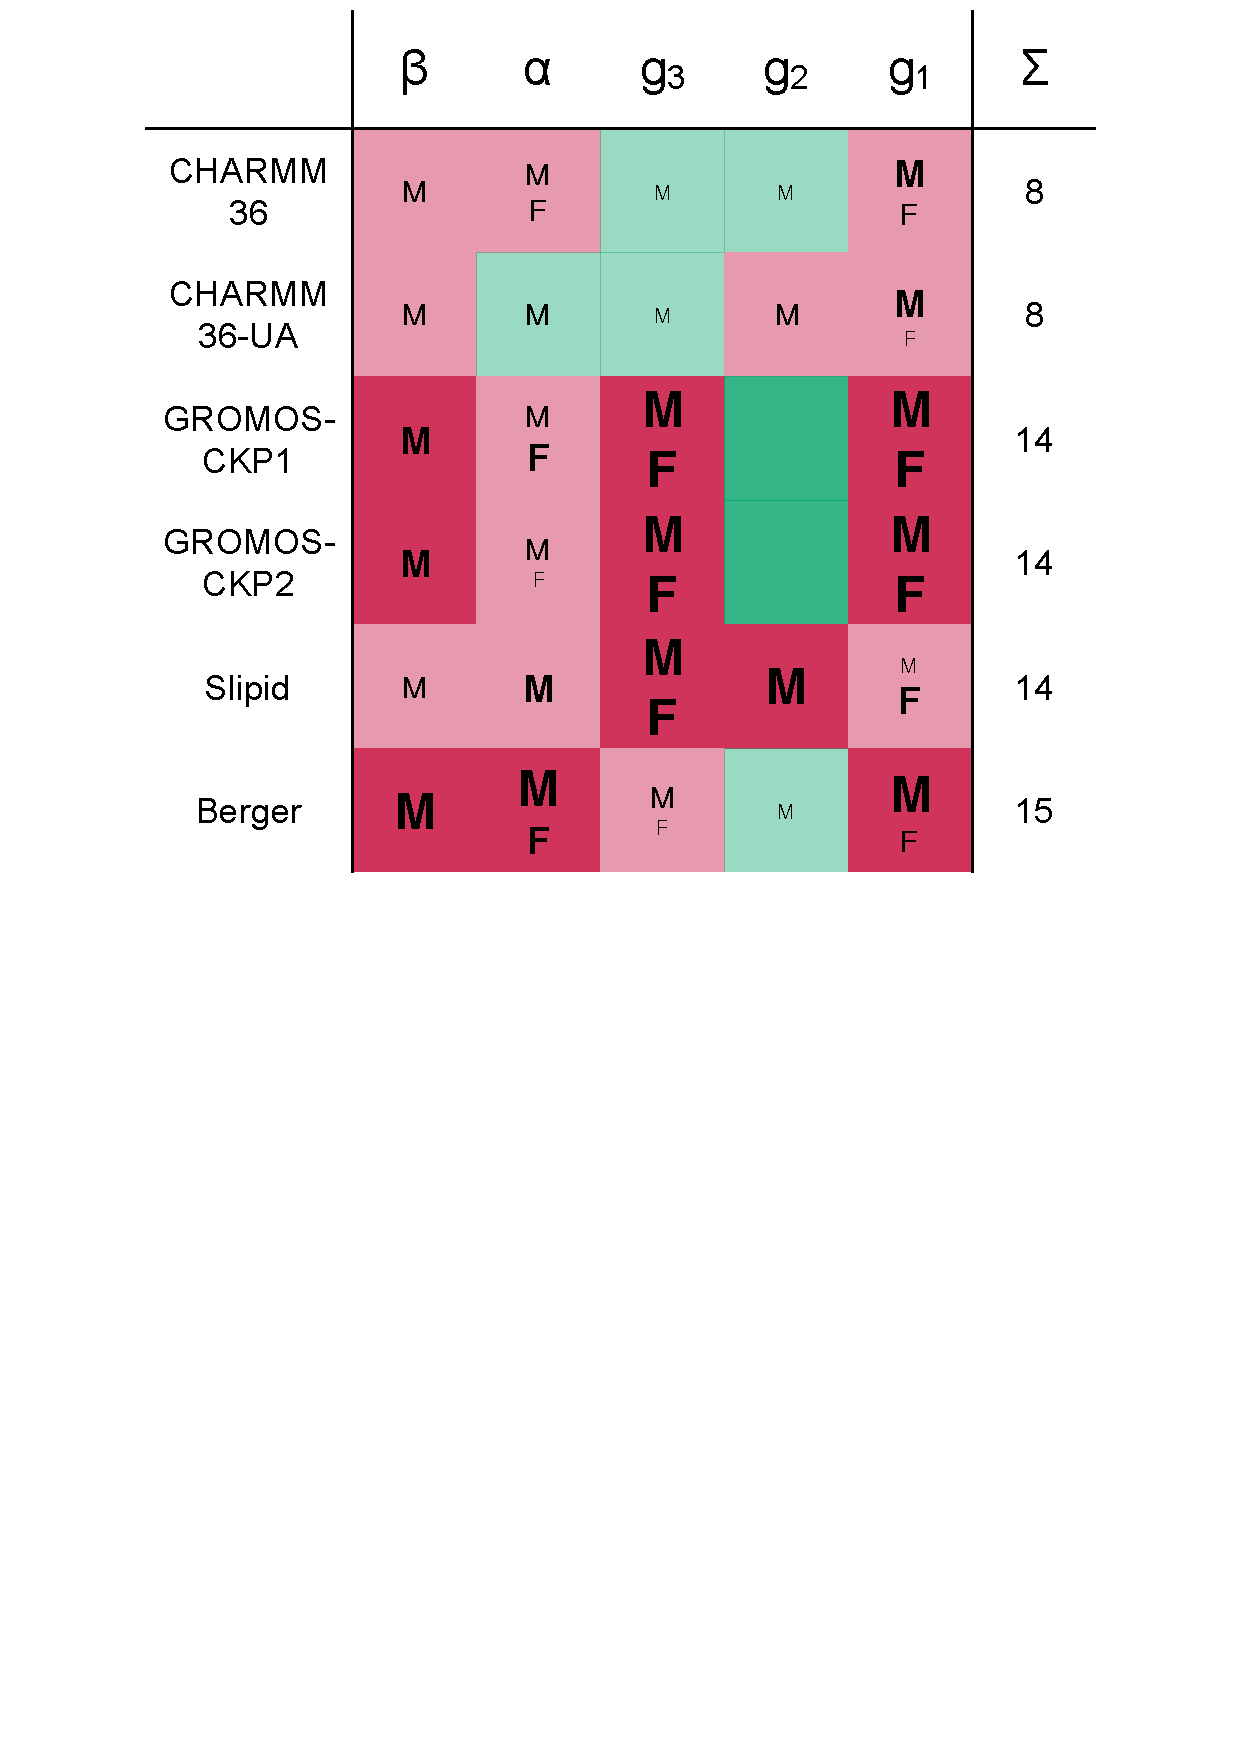
\includegraphics[width=9.0cm]{../Figs/comparisonTablePS.pdf}
  \caption{\label{comparisonTablePS}
  Rough subjective ranking of force fields based on Figure~\ref{HGorderParametersPS}. Here ÒMÓ indicates a magnitude problem, ÒFÓ a forking problem; letter size increases with problem severity. Color scheme: Òwithin experimental errorÓ (dark green), Òalmost within experimental errorÓ (light green), Òclear deviation from experimentsÓ (light red), and Òmajor deviation from experimentsÓ (dark red). The $\Sigma$-column shows the total deviation of the force field, when individual carbons are given weights of 0 (matches experiment), 1, 2, and 4 (major deviation). For full details of the assessment, see Supplementary Information.
  }
  \todo{Issue about possible updates to this plot: https://github.com/NMRLipids/NMRlipidsIVotherHGs/issues/4} \\
  \todo{Lipid17 and MacRog results should be added into this plot.}
\end{figure}

The headgroup order parameters of DOPS and POPS bilayers 
from different simulation models are compared with the experimental
data in Fig. \ref{HGorderParametersPS}. Subjective ranking
of the quality of the models is shown in Fig. \ref{comparisonTablePS}.
The tested models perform generally less well than in the previous
study for PC headgroup~\cite{botan15} and none of the models 
reproduce the experimental order parameters within
experimental error bars.
Therefore, the models cannot be straightforwardly used to interpret the
structure of PS headgroup. However, the differences between PC and PS headgroups
are partially reproduced by some of the models.

The two best performing models for the $\alpha$ and $\beta$-carbons of
PS, Slipids and CHARMM36, reproduce the large forking in the $\alpha$-carbon
and the Slipids model gives also a good agreement with experiments for
the $\beta$-carbon order parameter in both PC and PS headgroups
(Fig. \ref{HGorderParametersPS} and Ref.~\citenum{botan15}).
Interestingly, the dihedral angle distributions of CHARMM36
and Slipids in Fig.~\ref{dihedralsHG} share significant similarities
in the headgroup region. However, the experimental order parameters in the
glycerol backbone region are not well reproduced by the Slipids model,
which was also the case in for PC lipids \cite{botan15}.
This difference probably arises from the differences in
the dihedral angle distributions of C1-C2-C3-O31 and C2-C3-O31-C31
in Figure \ref{dihedralsGLY}, which are also illustrated in
Figure \ref{glycerol_buslaev}. 

%\todo{Discussion is to be finished.
%  One possible conclusion could be the following:
%  The main differences between the models in the headgroup region are observed
%  for dihedrals C12-C11-O12-P and C11-C12-C13-O1A.
%  CHARMM36, CHARMM36UA and Slipids give very similar results to the
%  dihedral C11-C12-C13-O1A, which is close to the $\beta$-carbon.
%  The order parameters of $\beta$-carbons for these three models
%  are in best argeement with the experiments in figure \ref{HGorderParametersPS}.
%  On the other hand, Gromos-CKP models give better order parameters
%  for $\alpha$-carbon than Slipids, CHARMM36 or CHARMM36UA. 
%  In conclusion, the suggestion would be that the single peak for
%  observed at 120 degrees in CHARMMs and Slipids would
%  be more realistic for C11-C12-C13-O1A dihedral, while the single peak at 180 degrees observed
%  in CKP models and in Berger would be most realistic for C12-C11-O12-P dihedral.
%}



\todo{Also the discussion about POPS/OPPS issue with MacRog model should be added.}

\begin{figure}[]
  \centering
  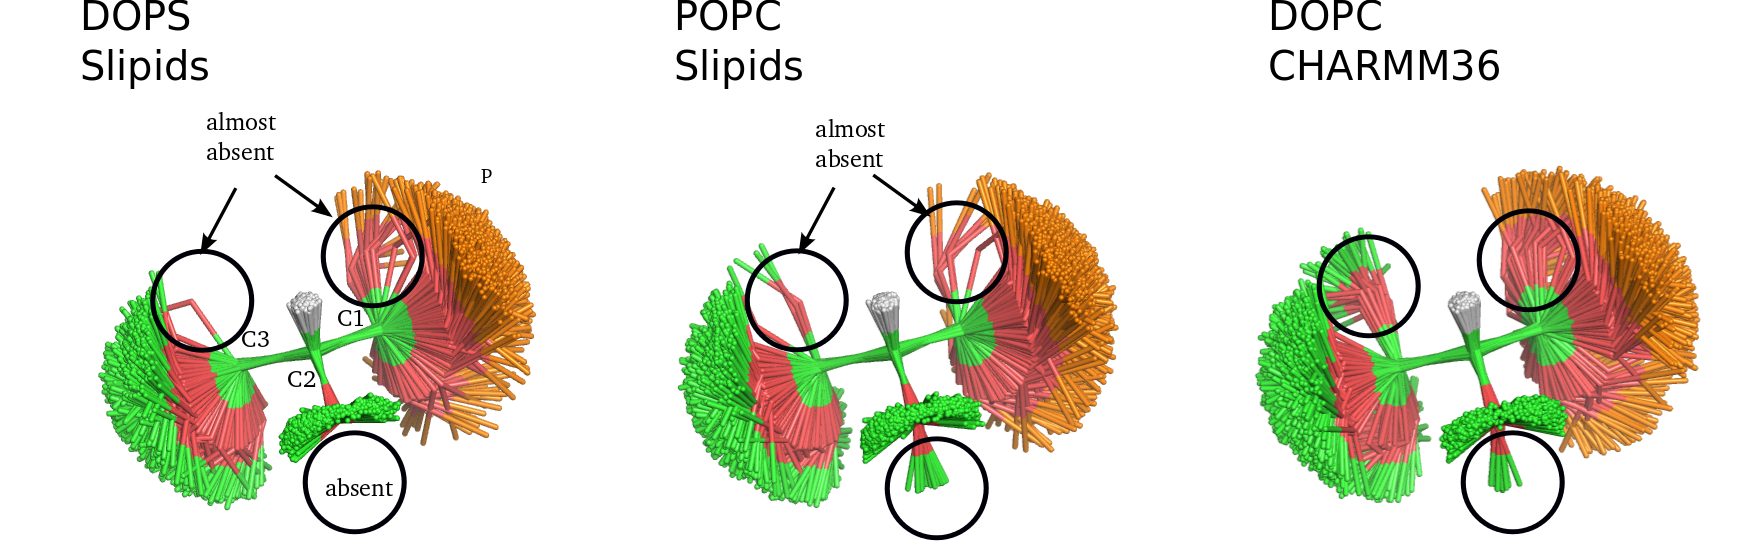
\includegraphics[width=9.0cm]{../Figs/glycerol_buslaev.png}
  \caption{\label{glycerol_buslaev}
    Snapshots overlayed from different simulations for glycerol backbone region
    by Pavel Buslaev.
  }
\end{figure}

%
%The total deviation from the experiments ($\Sigma$ in Fig. \ref{comparisonTablePS})
%for the best performing CHARMM36 model is larger for PS lipids (8)
%than for PC (3) \cite{botan15}.
%Therefore the interpretation of structural details of PS headgroup or
%differences between PC and PS lipids is very challenging 
%from the current MD simulation models.


\subsection{Counterion binding to lipid bilayers containing PS lipids}
Membranes containing PS lipids are always accomppanied with counterions, which
modulate electrostatic interactions between lipids and other biomolecules. 
Counterions are also suggested screen the repulsion between charged lipid headgroups 
in MD simulations and reduce the area per lipid of PS bilayers to be smaller than in PC
bilayers~\cite{pandit02,mukhopadhyay04,pedersen06}. 
The counterion density profiles along membrane normal 
show significant differences between simulation models (Fig. \ref{NAdensPOPS}).
The strongest counterion binding, i.e., the lowest concentrations in bulk water,
are observed in MacRog, Berger and Lipid17/JC simulations.
CHARMM36, CHARMM36ua and Gromos-CKP models exhibit two local maxima in counterion
density, while a single maxima is observed in the other models. 
\todo{More detailed discussion may be possible after comparing monovalent ion binding
to bilayers between CHARMM simulations and experiments.}
Area per lipid is in agreement with experiments \cite{pan14} only
in the Gromos-CKP models, while other models give significantly lower values (Fig. \ref{NAdensPOPS}).
The difference cannot be explained by the electrostatic screening of the headgroup repulsion due to 
counterion binding because CHARMM36, CHARMM36ua and Slipid models give
smaller area per lipid than Gromos-CKP models with similar counterion binding affinity.
%The proposed trend is observed for Lipid17 model,
%for which the Joung-Cheatham ions give higher affinity and smaller area
%per molecule. However, the trend is not observed when comparing accross different
%force fields. For example, CHARMM36ua and MacRog give similar area per molecule
%but binding affinity is significantly higher in MacRog. 
\begin{figure}[]
  \centering
  \includegraphics[width=9.0cm]{../Figs/NAdensPOPS.eps}
  \caption{\label{NAdensPOPS}
    Counterion densities of POPS lipid bilayer along the membrane normal from
    simulations with different force fields.
  }
\end{figure}

To evaluate counterion binding in different simulation models against experimental data~\cite{roux90},
we plot the headgroup order parameters measured from POPC:POPS 5:1 mixture
as a function of different monovalent ions added to the buffer (Fig. \ref{PSresponseTONaCl}). 
Experimental order parameter data for POPC headgroup in the mixture is available as a function
of LiCl and KCl concentrations, while POPS headgroup order parameters are measured also
as a function of NaCl. Lithium interacts more strongly with PS headgroups than other monovalent 
ions~\cite{hauser83,hauser85,roux86,mattai89,roux90}, as also observed for PC headgroups~\cite{cevc90}. 
This is evident also in the changes of PS headgroup order parameters, which decrease with the addition of lithium 
but increase with the addition of sodium or potassium (Fig. \ref{PSresponseTONaCl}). 
POPC headgroup order parameters exhibit a clear decrease as a function of LiCl concentration
but only modest changes as a function of KCl concentration, indicating singificant 
Li$^+$ binding but only weak Na$^+$ binding to the mixture when interpreted using the
electrometer concept~\cite{akutsu81,altenbach84,seelig87}. In simulations with the
Berger model, the headgroup order parameter response of POPC
to the added NaCl is similar to the experiments of LiCl,
indicating overestimated binding affinity of sodium, in line with the results for PC bilayers \cite{catte16}.
Indeed, the sodium density profile shows a significant binding peak in the 
Berger model (Fig. \ref{CIdensPSOCmixt}). Potassium binding in the MacRog simulation
is significantly weaker  (Fig. \ref{CIdensPSOCmixt}) and the headgroup order parameter 
changes are also in better agreement with simulations (Fig. \ref{PSresponseTONaCl}).
\todo{Discussion about Lipid17 to be written when we have the density profiles.}
All the tested models overestimate the changes of POPS headgroup order parameters as
a function of monovalent ions (Fig. \ref{PSresponseTONaCl}), suggesting that
model development is necessary to interpret the PS headgroup-ion interactions 
from MD simulations.
\begin{figure*}[]
  \centering
  \includegraphics[width=18.0cm]{../Figs/CHANGESwithMONVALENTwithPS.eps}
  \caption{\label{PSresponseTONaCl}
    Changes of the PC (left) and PS (right) headgroup order parameters as a function of
    added NaCl, KCl and LiCl from POPC:POPS (5:1) mixture. The experimental data is from Ref. \citenum{roux90}.
    The values from counterion-only systems are set as a zero point of y-axis.
    To correctly illustrate the significant forking of the $\alpha$-carbon order parameter
    in PS headgroup (bottom, right), the y-axis is tranferred with the same value for both order parameters such that the lower order
    parameter value is at zero.
  }
  \todo{CHARMM36 results for this plot would be highly useful.}
\end{figure*}


\begin{figure}[]
  \centering
  \includegraphics[width=8.0cm]{../Figs/CIdensPSOCmixt.eps}
  \caption{  Counterion density distributions from PC:PS mixtures.
\label{CIdensPSOCmixt}
  }
  \todo{Lipid 17 is to be added.}
\end{figure}




\subsection{Headgroup structure in PS and PC mixtures}
Dilution of PS lipid bilayers with PC lipids reduces propensity for the formation of
strong complexes with multivalent ions and is proposed to make PS headgroups 
less rigid~\cite{browning80,buldt81,roux90,roux91}. Therefore, the intermolecular
interactions at the headgroup region seems to determine important physical properties 
of mixed lipid bilayers. The headgroup order parameters of POPC increase in experiments 
with increasing amount of POPS in the mixed lipid bilayer (Fig.~\ref{HGorderparametersPCvsPS})~\cite{scherer87}. 
This behaviour is generally observed when negatively charged lipids or surfactants 
are mixed with PC lipids~\cite{scherer87,scherer89} and can be understood by the 
tilting of lipid headgroup more parallel to the membrane plane according to
the electrometer concept \cite{seelig87}. The headgroup order parameters of PS lipids
shift closer to zero when bilayer is diluted with PC lipids in 
experiments (Fig.~\ref{HGorderparametersPCvsPS})~\cite{browning80,scherer87,roux90},
which is intepreted to indicate reduced rigidity~\cite{browning80,buldt81}.

The increase of POPC headgroup order parameters with the increasing
amount of negatively charged POPS lipid is reproduced in
MacRog simulations with potassium counterions, but not in 
Berger simulations with sodium or in CHARMM36 simulations
with potassium or sodium conterions (Fig. \ref{HGorderparametersPCvsPS}). 
The observations can be explained using the electrometer concept.
The Berger simulation exhibits very strong sodium binding (Fig. \ref{CIdensPSOCmixt}), 
which surpasses the effect of negatively charged lipids as the amount of
counterions increase with increasing amount of PS.
In CHARMM36 simulations, the counterion binding neutralizes the effect
of PS and the headgroup order parameters are not changed with increasing amount
of PS. Finally, the weak binding of potassium in the MacRog simulations
enables the increase of order parameters with the added amount of PS 
(Figs. \ref{HGorderparametersPCvsPS} and \ref{CIdensPSOCmixt}).

\begin{figure*}[]
  \centering
  \includegraphics[width=16.0cm]{../Figs/HGorderparametersPCvsPS.eps}
  \caption{\label{HGorderparametersPCvsPS}
    Changes of PC (left panel) and PS (right panel) headgroup order parameters
    from POPC:POPS mixtures with increasing amount of POPS.
    Experimental results of POPC are taken from Ref. \citenum{scherer87}
    (signs are determined as discussed in \cite{botan15,ollila16}).
    Experimental values for POPS in pure bilayer and in mixture are  
    measured in this work and in Ref. \citenum{roux90} at 298K, respectively.
    Since the experimental data of POPS in pure and diluted mixture come from
    different experimental sets (13C NMR in this work and 2H NMR from Ref. \citenum{roux90}),
    the experimental change of the order parameter is less accurate than in typical measurements
    where same technique is used in all conditions, see discussion about qualitative and quantitative 
    accuracy in Ref. \citenum{ollila16}.
    For POPC (left panel) the zero point of y-axis is set to the value of pure bilayer.
    For $\beta$-carbon of POPS (right panel, top) the zero point of y-axis is
    set to the value from POPC:POPS (5:1) mixture.
    For $\alpha$-carbon of POPS (right panel, bottom) the y-axis is tranferred
    with the same value for both order parameters such that the lower order
    parameter value from POPC:POPS (5:1) mixture is at zero
    to correctly illustrate the significant forking.
  }
  \todo{Simulation of CHARMM36 at 298K should be maybe rerun with Gromacs 5.} \\
  \todo{Simulation of pure POPC at 298K with Lipid14 would be useful for this plot (only at 303 K is available from NMRlipids I)} \\
  \todo{MacRog simulations of pure POPS with potassium counterions only would be useful for this and other plots.}
\end{figure*}

Oppositely to experiments, the headgroup order parameter of POPS shift away
from zero in CHARM36 simulations when bilayer is diluted with POPC (Fig. \ref{HGorderparametersPCvsPS}).
In lipid14/17 simulations, the POPS order parameter shift closer to zero when
bilayer is diluted with POPC, but the numerical values of order parameters
are too far from experiments to enable interpretation of the experimental data.
Therefore, we conlcude that the force field development is necessary before
MD simulations can be used to interpret the interactions between PC and PS headgroups.
%The $\beta$-carbon order parameter
%increase with increasing amount of PS in CHARMM36 and MacRog simulations in contrast
%to the experimental data.
%The smaller $\alpha$-carbon order parameter increase in both
%simulation models with increasing amount of PS, while it is almost unchanged in experiments.
%The larger $\alpha$-carbon order parameter increase in MacRog and decrease in CHARMM36
%with increasing amount of PS, both model exhibiting a poor agreement with experiments. 



\subsection{Ca$^{2+}$ binding affinity in bilayers with negatively charged PS lipids}

%Also the Ca2+ binding affinity to bilayers containing
%PS lipids is measured from mixtures with PC, because pure PS
%bilayers exhibit instant transition to the ordered phase with the
%addition of the ions.
%Therefore, the characterization of mutual interactions
%between PC and PS lipid headgroups is necessary in order to
%understand PS lipids in biological environments.


The headgroup order parameters of PC lipids
decrease proportionally to the bound positive
charge in to a bilayer \cite{seelig87,catte16} and can be
therefore used to measure the ion binding
affinity. This molecular electrometer concept can
be also applied to lipid bilayers with mixtures
of PC and negatively charged lipids \cite{borle85,macdonald87,roux90}
(see Fig. \ref{OrderParameterCHANGESWithCaClBELOW1M}).
%This is demonstrated in Fig. %s \ref{OrderParametersWithCaCl},
%\ref{OrderParametersWithCaClBELOW1M} and
%using the previuosly reported experimental data
%for mixtures with varying proportions of
%negatively charged PS or PG lipids.
%
%the changes of PC headgroup order parameters %for PC headgroup $\alpha$ and $\beta$ carbons
%as a function of CaCl$_2$ concentration are shown
%
% (see Fig. \ref{OrderParameterCHANGESWithCaClBELOW1M}).



%PC headgroup order parameters increase when negatively charged
%PS or PG are added to PC bilayer in the absense of added CaCl$_2$,
%as expected based on electrometer concept \cite{seelig87}
%(see Fig. \ref{OrderParametersWithCaClBELOW1M}).
%In electrometer concept this is explained by the tilting of
%headgroup more parallel to membrane normal \cite{??}.

%Order parameters reach the values of pure PC bilayer close to CaCl$_2$ concentrations of $\sim$ 50-300mM.
%At this point the Ca2+ binding presumably fully cancels the charge from negative lipids and
%overcharging occurs above these concenterations.


The headgroup order parameter changes of POPC and POPS from POPC:POPS (5:1) mixtures
are shown in Fig. \ref{changesWITHCaClPS} as a function of Ca$^{2+}$ concentration from different
simulations and experiments \cite{roux90}. 
The ion density distributions from the simulations are shown in Fig. \ref{CAdensPCPSmixture}.
The results suggest that Ca$^{2+}$ ions clearly overbind in simulations with
MacRog and Berger models, as expected from previous results for PC lipid bilayers \cite{catte16}.
It should be noted, however, that the lowest concentration (100mM) gives
a good agreemet with experiments
\todo{Should be analyze/discuss this further?
  Binding with $\sim$100 mM is saturated in both Berger and MacRog simulations. Maybe this is realistic?
It should be noted that Berger simulation do not have counterions.}.
Surprisingly, the calcium binding seems to be too weak CHARMM36 simulations.
This is due to the NBfix interaction parameters from Ref. \citenum{kim16}, incorporated
in the parameters from CHARMM-GUI at the time of running the simulations (January 2018).
The binding of calcium to pure POPC bilayer is also too weak with these parameters
as shown in Figs. \ref{OP_CHARMM_CaCl_POPC_NBFix} and \ref{density_profile_CHARMM_CaCl_POPC_NBFix}.
\todo{The discussion is to be finished when we have all the data in the plot.}

\begin{figure*}[]
  \centering
  \includegraphics[width=18cm]{../Figs/CHANGESwithCaClPS.eps}
  \caption{\label{changesWITHCaClPS}
    Changes of POPC (left) and POPS (right) headgroup order parameters in POPC:POPS (5:1) mixture
    as a function CaCl$_2$ concentration. Experimental data is taken from \citenum{roux90}.
    The values from counterion-only systems are set as a zero point of y-axis.
    To correctly illustrate the significant forking of the $\alpha$-carbon order parameter
    in PS headgroup (bottom, right), the y-axis is tranferred with the same value for both order parameters such that the lower order
    parameter value is at zero. 
  }
  \todo{Information about the cuonterions in different simulations should be added} \\
  \todo{Upcoming simulations with original CHARMM36 have been mentioned in the blog:
  http://nmrlipids.blogspot.com/2017/12/nmrlipids-iv-current-status-and.html?showComment=1520090718976\#c5569269391707740056} \\
  \todo{Upcoming Lipid17 simulations have been mentioned in the blog
    http://nmrlipids.blogspot.com/2017/12/nmrlipids-iv-current-status-and.html?showComment=1515177306419\#c994825612316235467}
\end{figure*}
\begin{figure}[]
  \centering
  \includegraphics[width=9cm]{../Figs/CAdensPCPSmixture.eps}
  \caption{\label{CAdensPCPSmixture}
    Ca2+ density profiles from simulations.
  }
  \todo{The CHARMM results are mass densities, numbers should be used.} \\
  \todo{Should we include also counterions into the plot?} \\
  \todo{Not all the data from MacRog is included.} 
\end{figure}


Also the order parameters of PS headgroup from POPC:POPS (5:1) mixture
are shown in Fig. \ref{changesWITHCaClPS} as a function of CaCl$_2$ concentration.
In experiments the order parameters exhibit a strong dependence of CaCl$_2$ with
small concentrations with a rapid saturation around 50 mM. 
The changes of PS headgroup order parameters with added CaCl$_2$ are overestimated in
all tested simulation models. Furthermore, the changes of the headgroup order parameters
do not qualitatively agree with experiments. This is in contrast to previous results
for PC headgroup \cite{catte16}, where qualitatively correct reponse to bound ions was
observed despite of significant discrepancies in the headgroup structure without additional ions. 


\section{Conclusions}


% Tables may be be put in the text as floats.
% Here is an example of the general form of a table:
% Fill in the caption in the braces of the \caption{} command. Put the label
% that you will use with \ref{} command in the braces of the \label{} command.
% Insert the column specifiers (l, r, c, d, etc.) in the empty braces of the
% \begin{tabular}{} command.
%
% \begin{table}
% \caption{\label{} }
% \begin{tabular}{}
% \end{tabular}
% \end{table}

% If you have acknowledgments, this puts in the proper section head.
\begin{acknowledgments}
% Put your acknowledgments here.
\end{acknowledgments}
\pagebreak
\appendix
\begin{center}
{\bf SUPPLEMENTARY INFORMATION}
\end{center}

\section{Simulated systems}

\subsection{CHARMM36}
\todo{To be written by Piggot, Madsen and Ollila}

\subsection{CHARMM36ua}
\todo{To be written by Piggot}

\subsection{Slipids}
\todo{To be written by Piggot and Favela}

\subsection{Berger}
\todo{To be wiritten by Piggot and Ollila}
Simulations with sodium were taken directly from Ref. \citenum{??} and
simulations with calcium directly from \citenum{melcrova16}.
Simulation of POPC at 310 K was taken directly from Ref. \citenum{ollila07a}.

\subsection{GROMOS-CKP}
\todo{To be written by Piggot}

\subsection{Lipid17}
\todo{To be written by Kav and Miettinen}

\subsection{MacRog}
\todo{To be written by Javanainen and Piggot}


\section{Cation binding affinity to lipid bilayers with different amount of charge}

%\begin{figure}[]
%  \centering
%  \includegraphics[width=9.0cm]{../Figs/LIPIDSwithCaCl.eps}
%  \caption{\label{OrderParametersWithCaCl}
%    PC headgroup order parameters as a function of CaCl concentration from experiments containing charged lipids.
%    Pure DPPC data from \cite{akutsu81}, pure POPC data from \cite{altenbach84}, 
%    POPC:POPS mixture data from \cite{roux90}, POPC:POPG mixture data with 0.1M NaCl from \cite{macdonald87}
%    and POPC:POPG mixture data without NaCl from \cite{borle85}.
%  }
%  \todo{Check the NaCl concentrations in the samples.}
%\end{figure}
%\begin{figure}[]
%  \centering
%  \includegraphics[width=9.0cm]{../Figs/LIPIDSwithCaClBELOW1M.eps}
%  \caption{\label{OrderParametersWithCaClBELOW1M}
%    Figure \ref{OrderParametersWithCaCl} zoomed to smaller concentrations.
%  }
%\end{figure}
\begin{figure}[]
  \centering
  \includegraphics[width=9.0cm]{../Figs/CHANGESwithCaCl.eps}
  \caption{\label{OrderParameterCHANGESWithCaClBELOW1M}
    The change of PC headgroup order parameters as a function of CaCl$_2$
    measured from bilayers containing different amount of negatively charged lipids.
    The values are taken from 2H NMR experiments reported in the
    literature (DPPC \cite{akutsu81}, POPC \cite{altenbach84}, POPC:POPS (5:1) \cite{roux90},
    POPC:POPG  mixtures with 0.1M NaCl \cite{macdonald87}
    and POPC:POPG (1:1) without NaCl \cite{borle85}).
    As expected, the decrease of order parameters with the added CaCl$_2$
    is more pronounced for systems with larger fraction of
    negatively charged lipids, indicating larger amount amount
    of bound cations.
  }
\end{figure}



Before using the headgroup order parameters to compare ion binding affinity between simulations
and experiments, it is important to quantify the response of the order parameters to the
bound charge in simulations.
The response of headgroup order parameters to the fixed amount of cationic surfactants in
POPC bilayer is compared between simulations and experiments \cite{scherer89} In Fig. \ref{CHANGESwithCaClPGPS}.
The figure shows that the order parameters are too sensitive to bound charge in Lipid14 model,
while CHARMM36 is in better agreement with experiments. This has to be taken into account when
analysin the binding affinities.
\begin{figure}[]
  \centering
  \includegraphics[width=9.0cm]{../Figs/HGopsDHMDMAB.eps}
  \caption{\label{CHANGESwithCaClPGPS}
  The response of headgroup order parameters to the fixed amount of cationic surfactants in
  POPC bilayer is compared between simulations and experiments \cite{scherer89}.}
\end{figure}

\section{Difference between POPC and OPPS in MacRog model}

\begin{figure}[]
  \centering
  \includegraphics[width=9.0cm]{../Figs/HGorderparametersPOPSvsOPPS.eps}
  \caption{\label{CHANGESwithCaClPGPS}
    Headgroup order parameters from POPS and OPPS simulations with MacRog model.}
\end{figure}

\section{Dihedrals}
\begin{figure*}[]
  \centering
  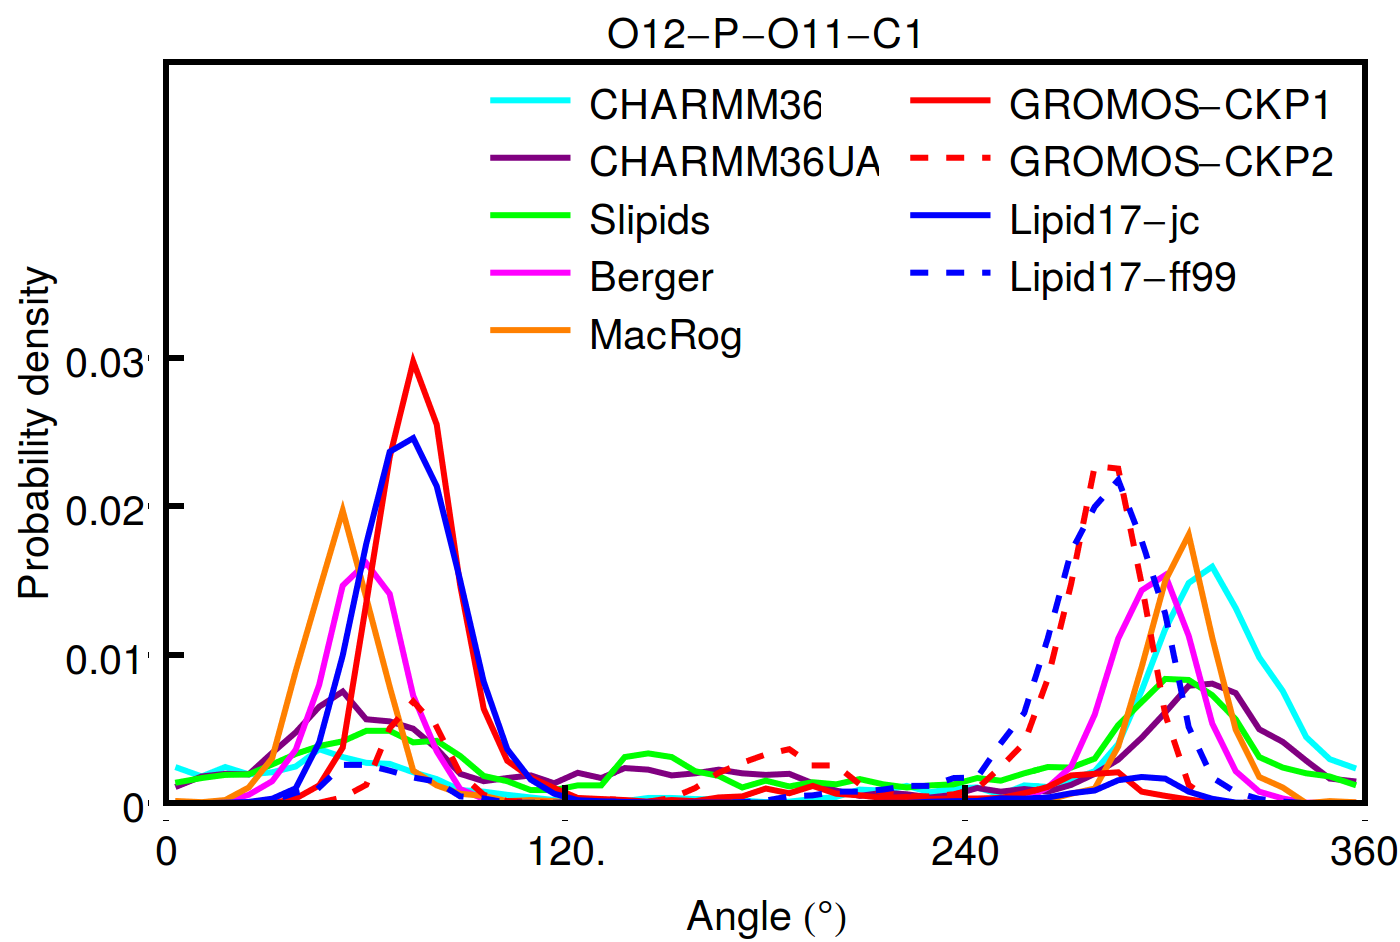
\includegraphics[width=8.0cm]{../Figs/diheds_pops1.png}
  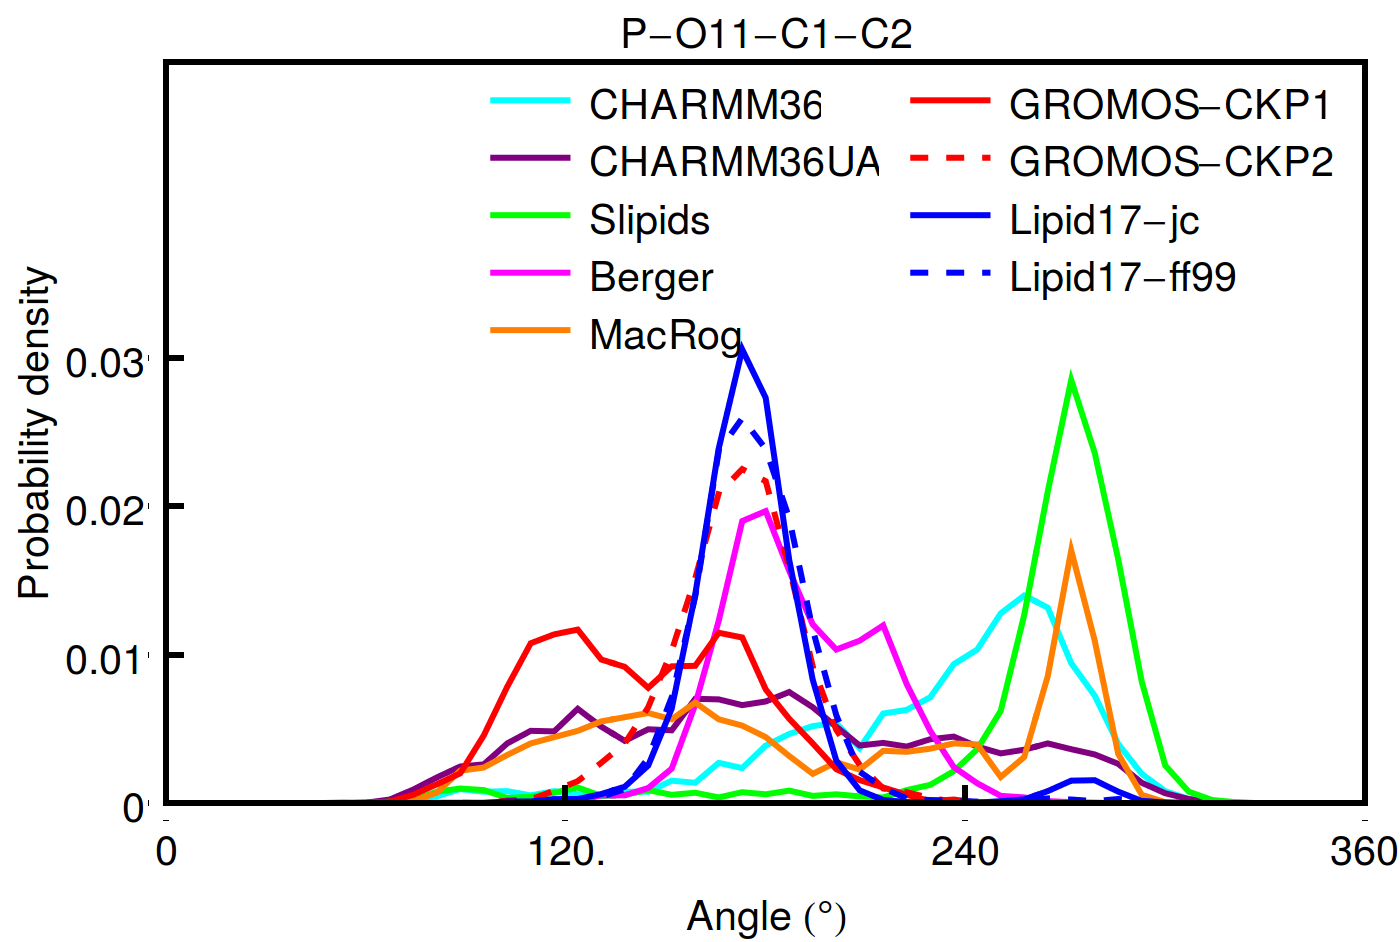
\includegraphics[width=8.0cm]{../Figs/diheds_pops2.png}
  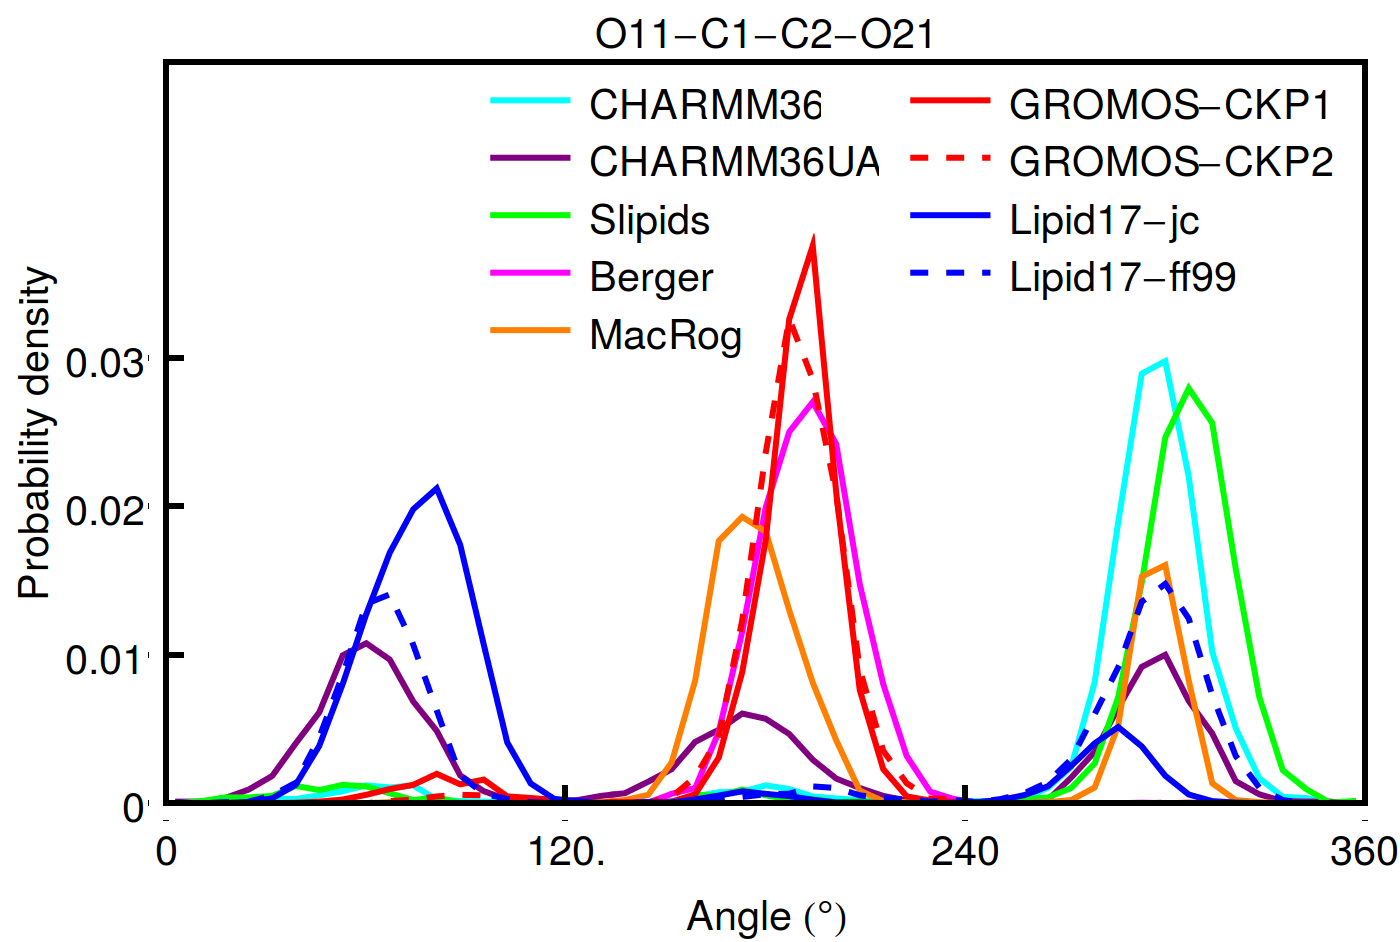
\includegraphics[width=8.0cm]{../Figs/diheds_pops3.png}
  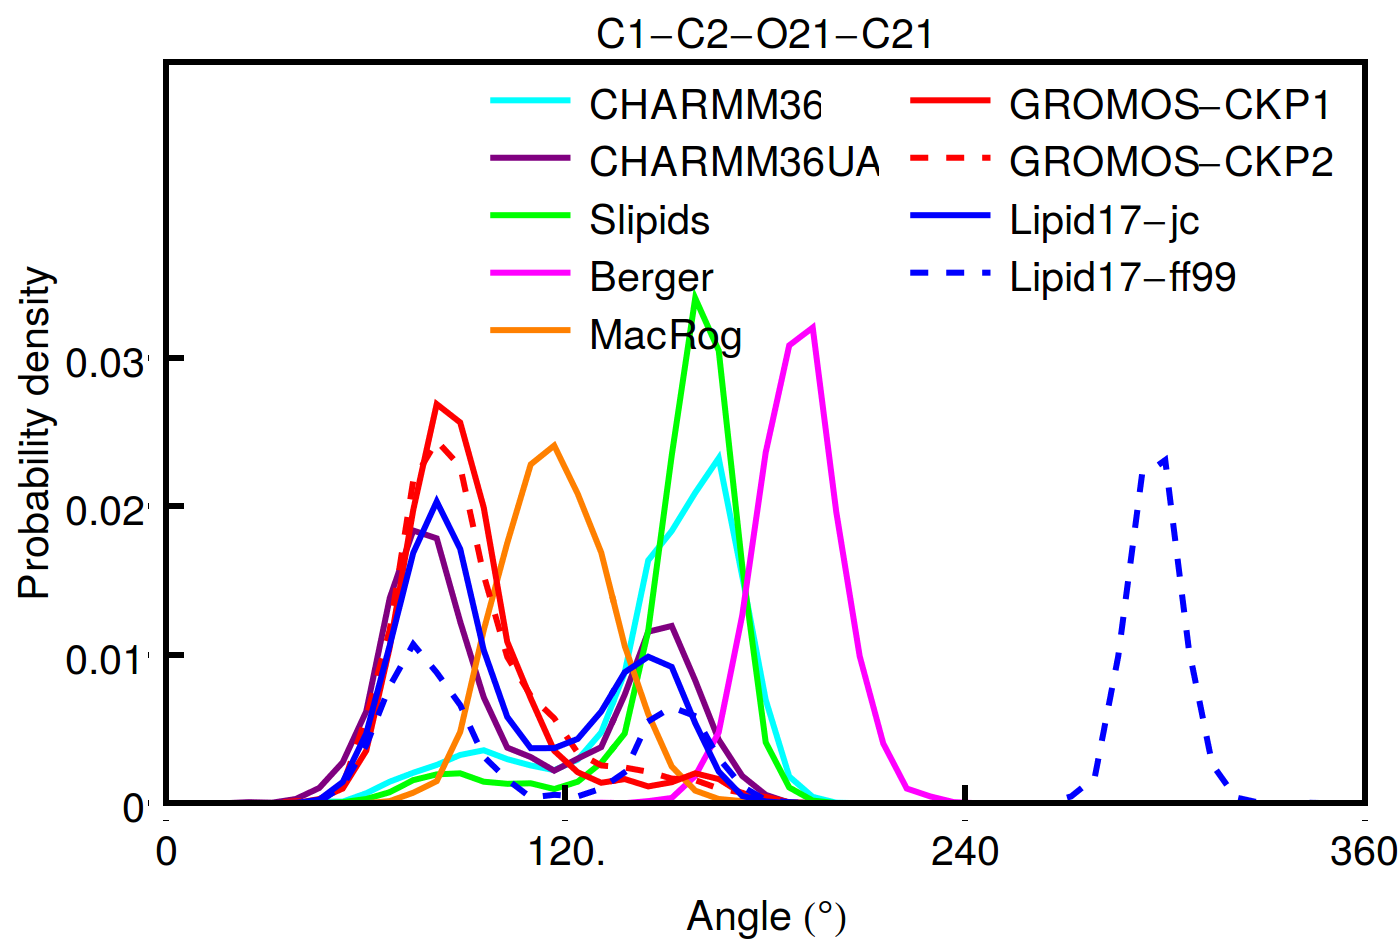
\includegraphics[width=8.0cm]{../Figs/diheds_pops4.png}
  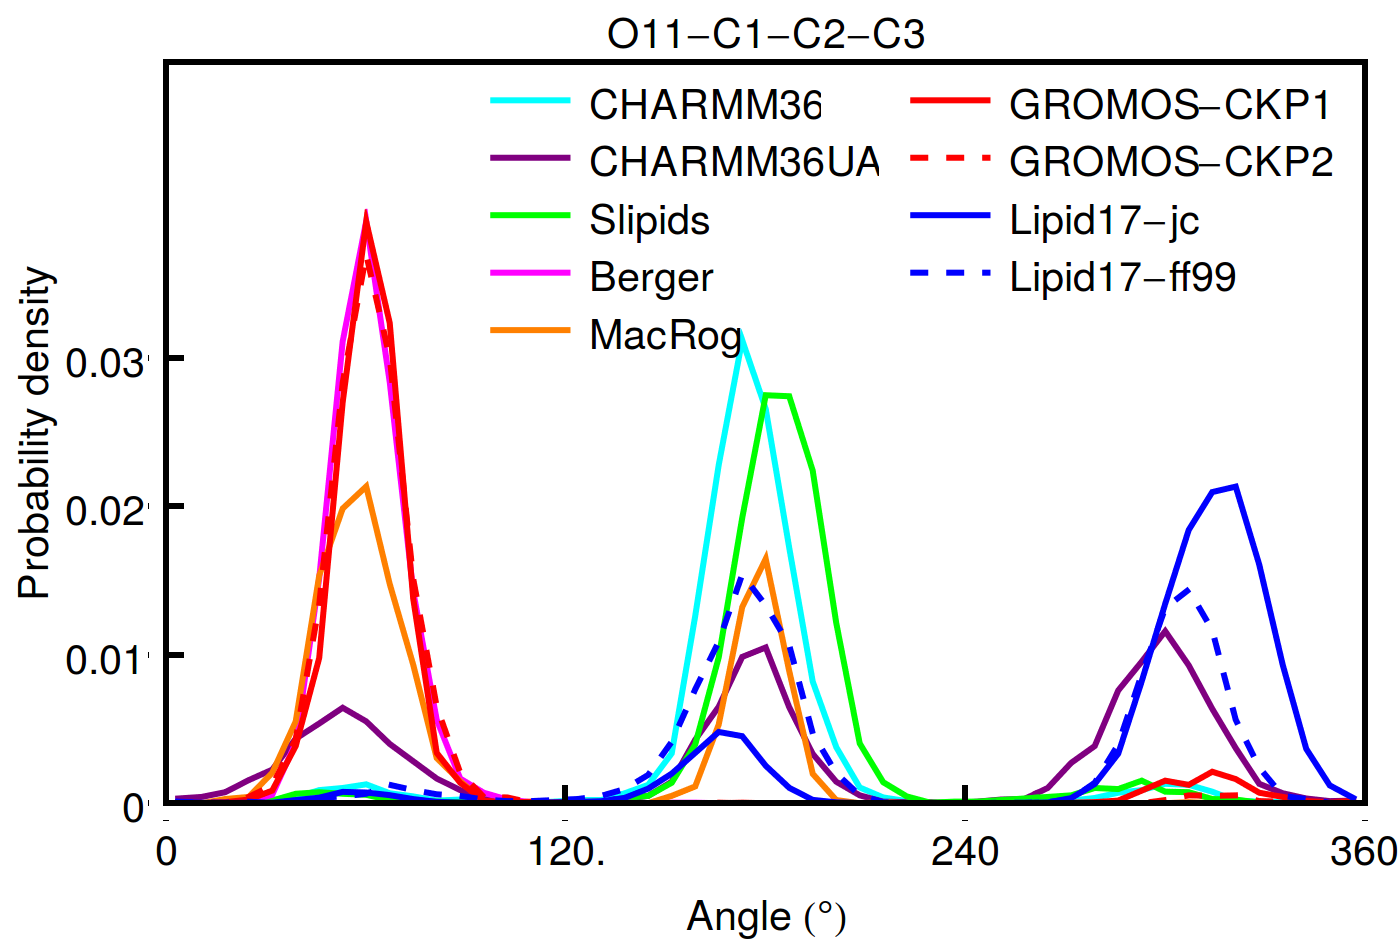
\includegraphics[width=8.0cm]{../Figs/diheds_pops5.png}
  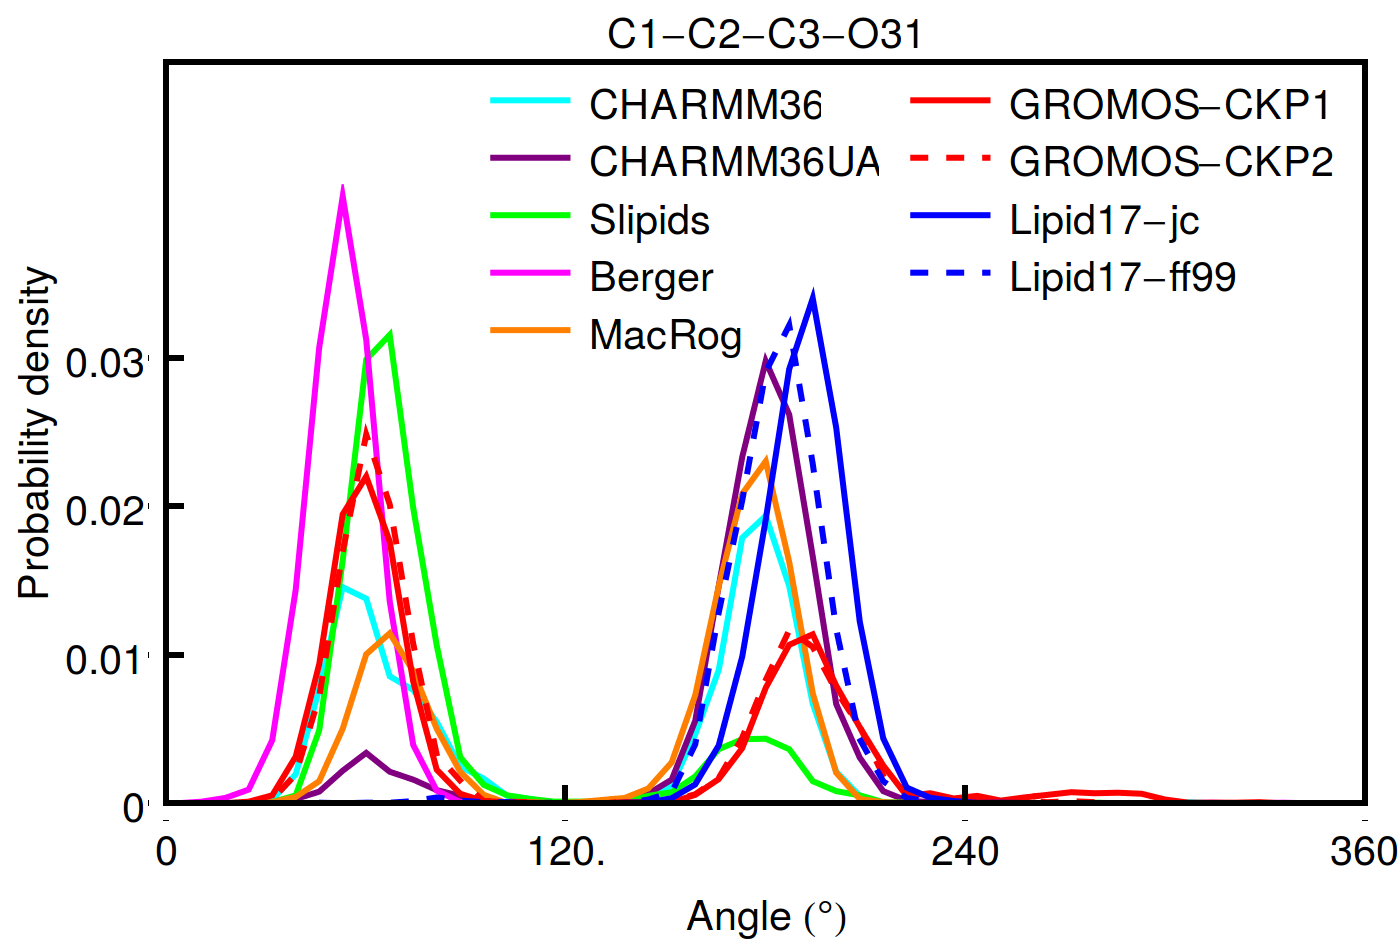
\includegraphics[width=8.0cm]{../Figs/diheds_pops6.png}
  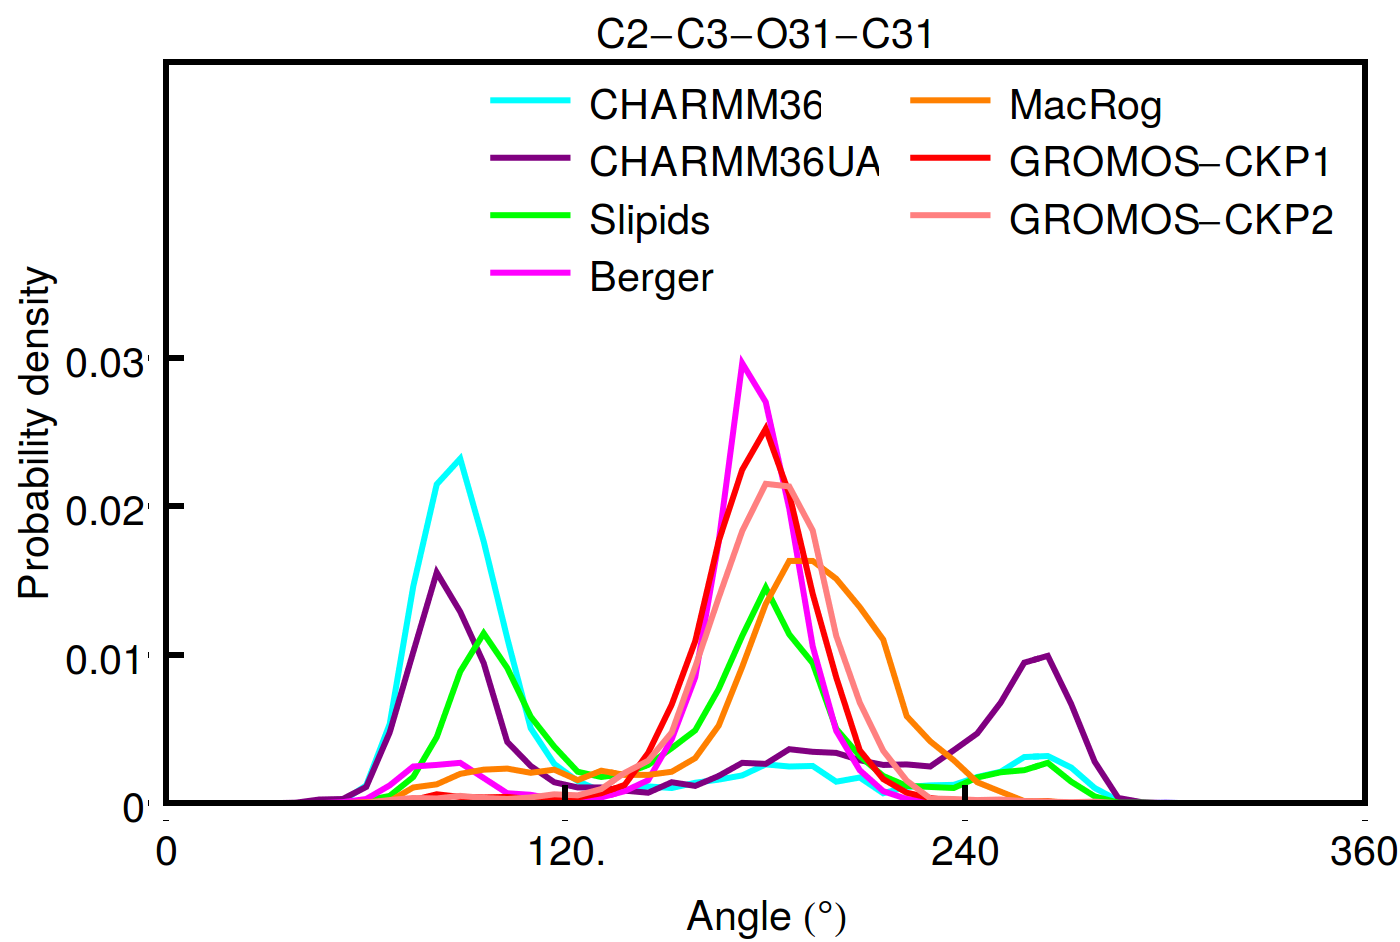
\includegraphics[width=8.0cm]{../Figs/diheds_pops7.png}
  \caption{\label{dihedralsGLY}
    Dihedral angle distributions of bonds from phosphate to acyl chain carbonyls from different simulation models.
  }
\end{figure*}
\section{Dihedrals}
\begin{figure*}[]
  \centering
  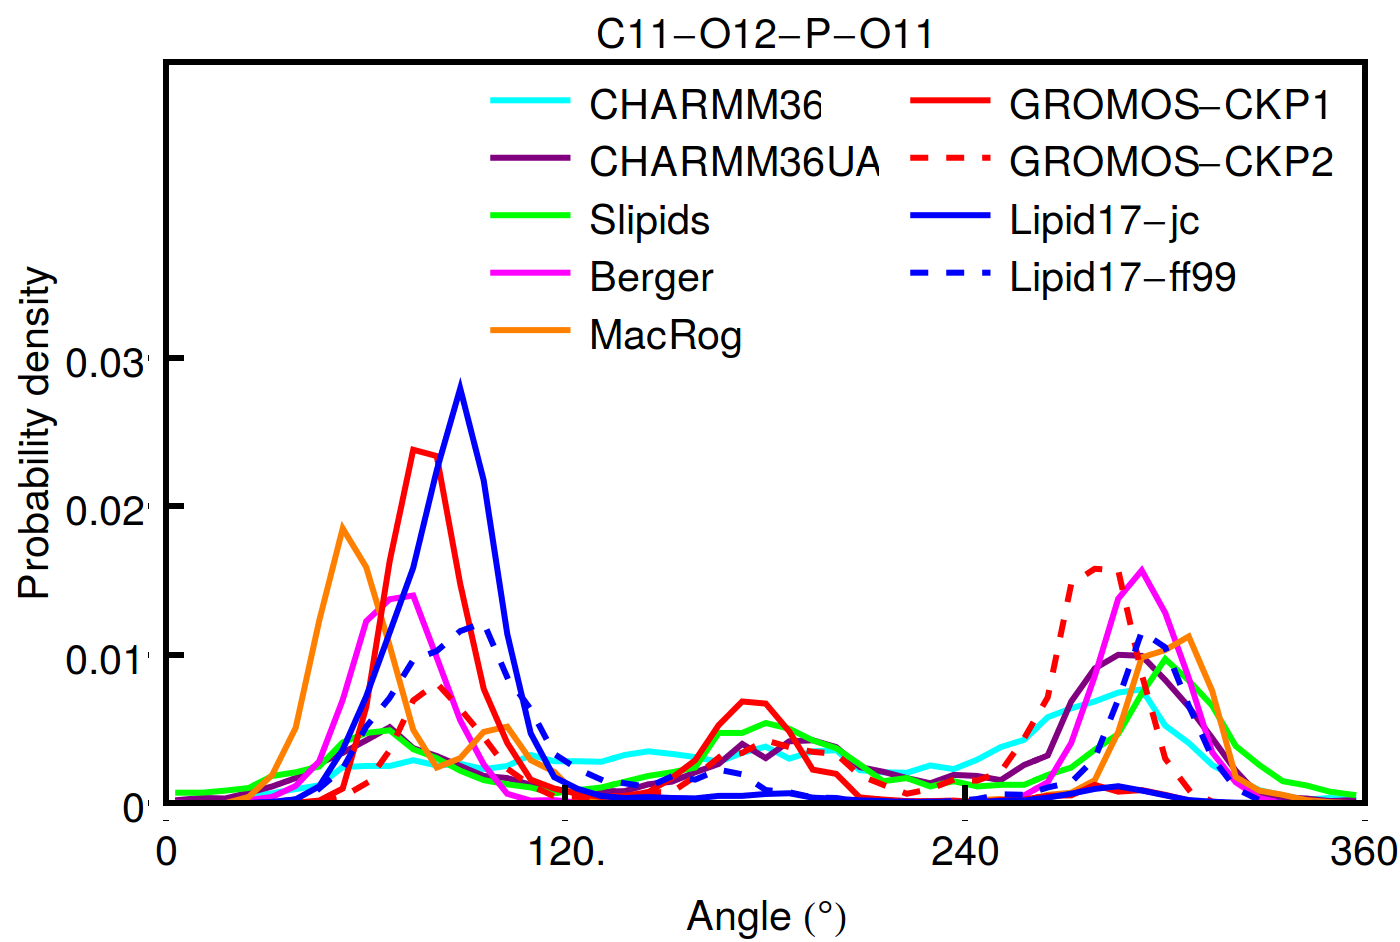
\includegraphics[width=8.0cm]{../Figs/diheds_pops8.png}
  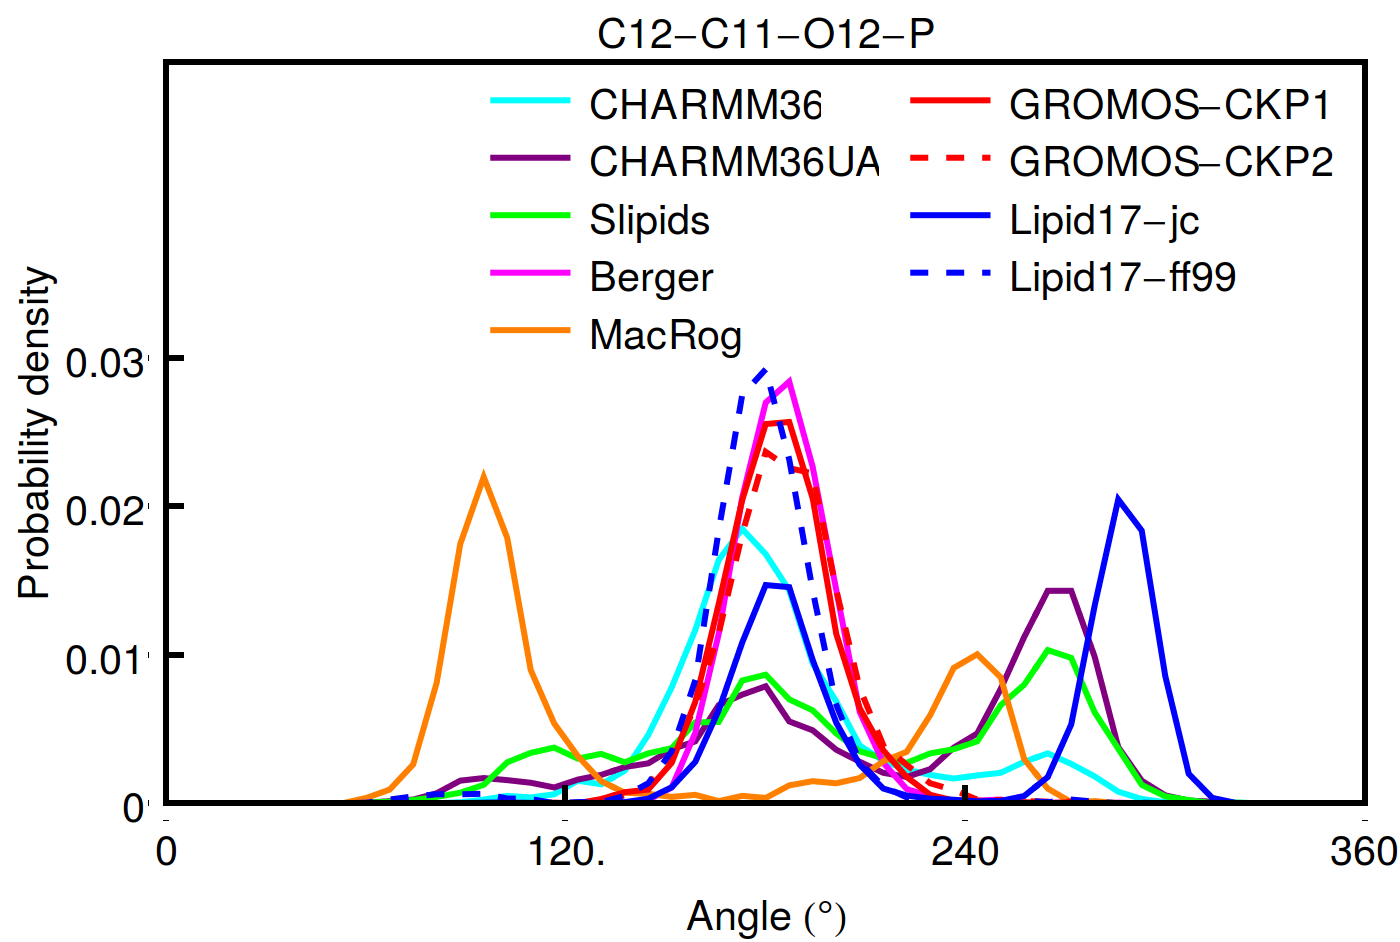
\includegraphics[width=8.0cm]{../Figs/diheds_pops9.png}
  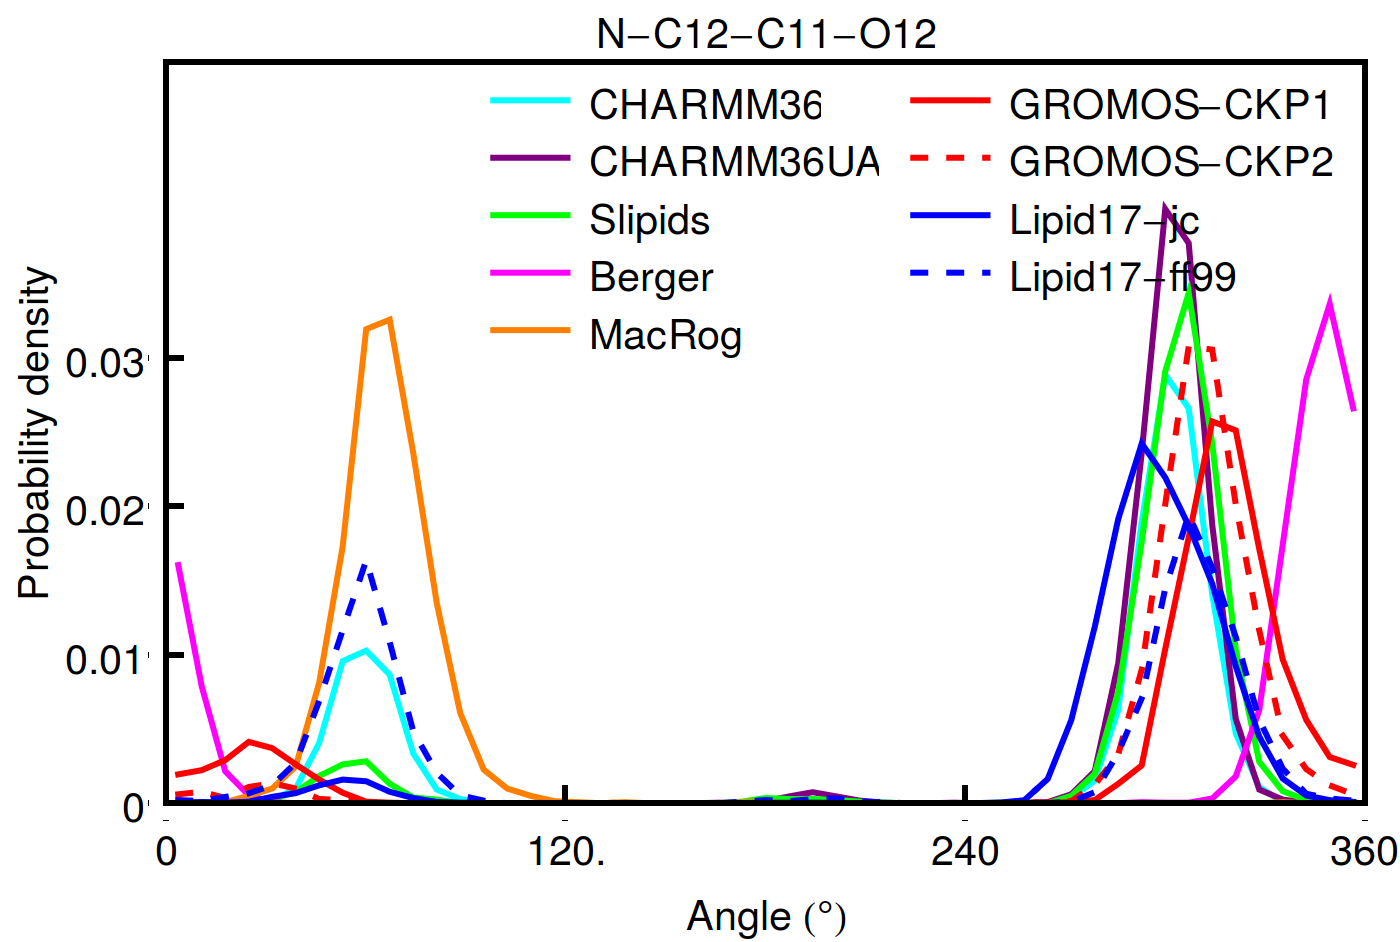
\includegraphics[width=8.0cm]{../Figs/diheds_pops10.png}
  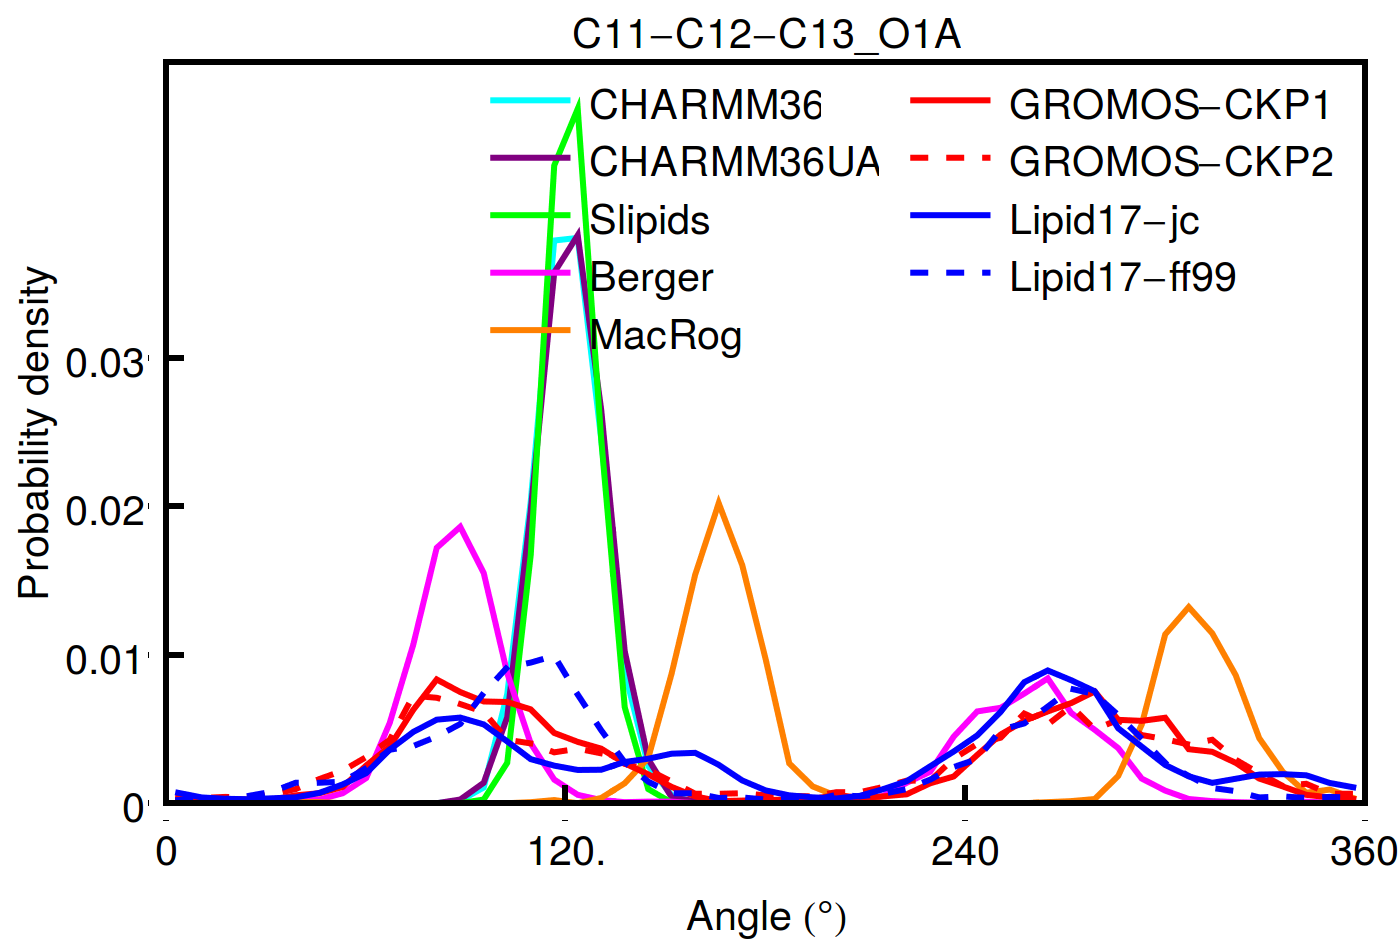
\includegraphics[width=8.0cm]{../Figs/diheds_pops11.png}
  \caption{\label{dihedralsHG}
    Dihedral angle distributions of bonds from phosphate to headgroup from different simulation models.
  }
\end{figure*}

\begin{figure}[]
  \centering
  \includegraphics[width=9.0cm]{../Figs/PSresponseTONaCl.eps}
  \caption{\label{PSresponseTONaClDMPC}
    Order parameters of PS headgroup as a function of added NaCl measured from DMPC:DMPS (3:1) mixture \cite{roux86}.
  }
\end{figure}
The experimental results show essentially no changes in the order parameters as a function of
added NaCl, while significant changes are observed in simulations. However,
the minimum buffer concentration of NaCl in the experimental was 100mM \cite{roux86}.
Therefore, we cannot exclude the possibility that the NaCl induced changes were already
saturated with 100mM NaCl concentration, which was the case for CaCl$_2$ in Fig. \ref{changesWITHCaClPS}.



\begin{figure}[]
  \centering
  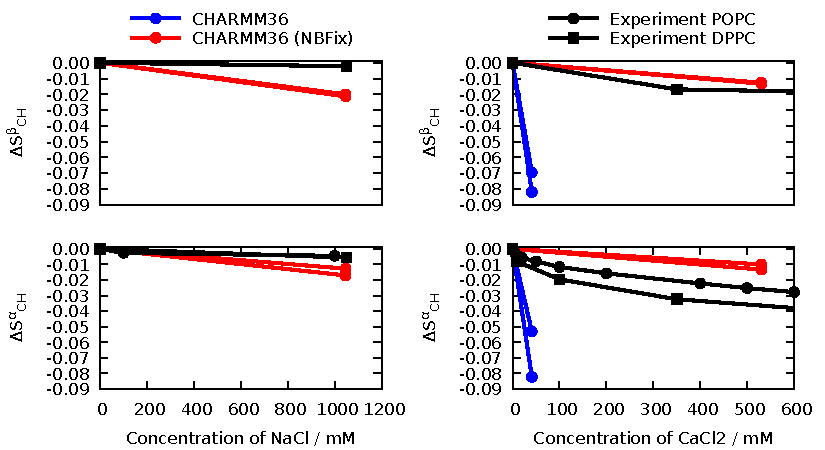
\includegraphics[width=9.0cm]{../Figs/OP_CHARMM_CaCl_POPC_NBFix.pdf}
  \caption{\label{OP_CHARMM_CaCl_POPC_NBFix}
  The response of headgroup order parameters to the fixed amount of cationic surfactants in
  POPC bilayer is compared between simulations and experiments \cite{scherer89}.}
\end{figure}

\begin{figure}[]
  \centering
  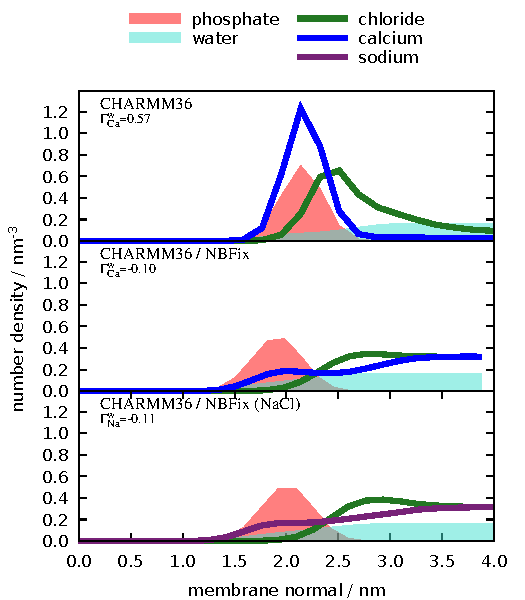
\includegraphics[width=9.0cm]{../Figs/density_profile_CHARMM_CaCl_POPC_NBFix.pdf}
  \caption{\label{density_profile_CHARMM_CaCl_POPC_NBFix}
  The response of headgroup order parameters to the fixed amount of cationic surfactants in
  POPC bilayer is compared between simulations and experiments \cite{scherer89}.}
\end{figure}

\pagebreak
\section{Details of the rough subjective force field ranking (Fig.~\ref{comparisonTablePS})} 

The assessment was based fully on the Fig.~\ref{HGorderParametersPS}.
%
First, for each carbon (the columns in Fig.~\ref{HGorderParametersPS}) in each force field (the rows),
we looked separately at deviations in magnitude and forking.

{\bf Magnitude} deviations, i.e., how close to the experimentally obtained C--H order parameters (OPs)
the force-field-produced OPs were.
%
For each carbon, the following 5-step scale was used:
%
\begin{description}
\item [0 (~):] \noindent {More than half of all the calculated OPs (that is, of all different hydrogens in all different lipids) were within the {\it subjective sweet spots} (SSP, blue-shaded areas in Fig.~\ref{HGorderParametersPS}).}
%
\item [1 ({\textsf{\tiny M}}):] \noindent {All the calculated OPs  were $< 0.03$ units away from the SSP.}
%
\item [2  ({\textsf{\small M}}):] \noindent {All the calculated OPs  were $< 0.05$ units away from the SSP.}
%
\item [3 ({\textsf{\large M}}):] \noindent {All the calculated OPs  were $< 0.10$ units away from the SSP.}
%
\item [4 ({\textsf{\Large M}}):] \noindent {Some of the calculated OPs  were $> 0.10$ units  away from the SSP.}
\end{description}

{\bf Forking} deviations, i.e., how well the difference in order parameters of two hydrogens attached to a given carbon matched that obtained experimentally. Note that this is not relevant for $\beta$ and $\mathrm{g_2}$, which have only one hydrogen. For the $\alpha$ carbon,  for which a considerable forking of 0.105 is experimentally seen, the following 5-step scale was used:
\begin{description}
\item [0 (~):] \noindent {The distance $D$ between the dots (that mark the measurement-time-weighted averages in Fig.~\ref{HGorderParametersPS}) was $0.08 < D< 0.13$ units for all the calculated OPs (that is, for all different lipids).}
%
\item [1 ({\textsf{\tiny F}}):] \noindent {$(0.06 < D < 0.08)$ OR $(0.13 < D < 0.15)$.}
%
\item [2  ({\textsf{\small F}}):] \noindent {$(0.04 < D < 0.06)$ OR $(0.15 < D < 0.17)$.}
%
\item [3 ({\textsf{\large F}}):] \noindent {$(0.02 < D < 0.04)$ OR $(0.17 < D < 0.19)$.}
%
\item [4 ({\textsf{\Large F}}):] \noindent {$(D<0.02)$ OR $(0.19<D)$.}
\end{description}
%
For the $\mathrm{g_3}$ carbon, for which no forking is indicated by experiments, the following 5-step scale was used:
%
\begin{description}
\item [0 (~):] \noindent {$ D< 0.02$.}
%
\item [1 ({\textsf{\tiny F}}):] \noindent {$0.02 < D < 0.04$.}
%
\item [2  ({\textsf{\small F}}):] \noindent {$0.04 < D < 0.06$.}
%
\item [3 ({\textsf{\large F}}):] \noindent {$0.06 < D < 0.08$.}
%
\item [4 ({\textsf{\Large F}}):] \noindent {$0.08 < D$.}
\end{description}
%
For the $\mathrm{g_1}$ carbon, for which a considerable forking of 0.13 is experimentally seen, the following 5-step scale was used:
%
\begin{description}
\item [0 (~):] \noindent {$0.11 < D < 0.15$.}
%
\item [1 ({\textsf{\tiny F}}):] \noindent {$(0.09 < D < 0.11)$ OR $(0.15 < D < 0.17)$.}
%
\item [2  ({\textsf{\small F}}):] \noindent {$(0.07 < D < 0.09)$ OR $(0.17 < D < 0.19)$.}
%
\item [3 ({\textsf{\large F}}):] \noindent {$(0.05 < D < 0.07)$ OR $(0.19 < D < 0.21)$.}
%
\item [4 ({\textsf{\Large F}}):] \noindent {$(D<0.05)$ OR $(0.21<D)$.}
\end{description}

Based on these assessments of magnitude and forking deviations,
each carbon was then assigned to one of the following groups:
"within experimental error"
(magnitude and forking deviations both on step 0 of the scales described above),
"almost within experimental error"
(sum of the magnitude and forking deviation steps 1 or 2),
"clear deviation from experiments"
(sum of magnitude and forking deviation steps from 3 to 5), and
"major deviation from experiments"
(sum of magnitude and forking deviation steps from 6 to 8).
These groups are indicated by colors in Fig.~4.
(Note that for $\beta$ and $\mathrm{g_2}$, for which there can be no forking,
the corresponding group assigment limits were: 0, 1, 2, and 3.)

Finally, the total ability of the force field to describe the headgroup and
glycerol structure was estimated.
To this end, the groups were given the following weights:
0 (within experimental error),
1 (almost within experimental error),
2 (clear deviation from experiments),
4 (major deviation from experiments),
and the weights of the five carbons were summed up.
The sum, given in the $\Sigma$-column of Fig.~\ref{HGorderParametersPS},
was then used to (roughly and subjectively, as should be clear from the
above description) rank the force fields.

\newpage


% Create the reference section using BibTe
\bibliography{refs.bib}

%\newpage
%\section{APPENDIX: The NMR results reported by Tiago Ferreira}

\listoftodos

\end{document}
%
% ****** End of file aiptemplate.tex ******
